%!TEX root = ../Systementwurf.tex

\chapter{Analyse der Produktfunktionen}\label{chap:analyse}

In diesem Kapitel werden die im Pflichtenheft vorgestellten Produktfunktionen
und ggf. die nicht-funktionalen Anforderungen analysiert und in
Sequenzdiagrammen dargestellt.
So wird gut erkennbar, welche Nachrichten die einzelnen Komponenten von \NewsGenie austauschen und welche
Funktionen aufgerufen werden um die jeweilige Funktion zu realisieren.
Dies dient als Basis um eine geeignete Architektur zu wählen.


\section{Analyse von Funktionalität \ref{F10}: Sprachausgabe}

\NewsGenie kommuniziert über gesprochene Sprache mit dem Nutzer. Wenn eine
Sprachausgabe auf dem Client erfolgen soll, wird wie in Abb.~\ref{sd10} dargestellt vom \textit{ManagementHandler}, der für die Kommunikation
von Client und Server zuständig ist, ein \textit{ClientAnswer}-Objekt an den
Client gesendet.
Der Client ruft daraufhin die Funktion \textit{Say.text()} auf und übergibt den im
\textit{ClientAnswer}-Objekt gespeicherten String an die Funktion. Diese wandelt
ihn in eine Wave-Datei um und spielt diese für den Nutzer ab.

\begin{figure}[h]
\centering
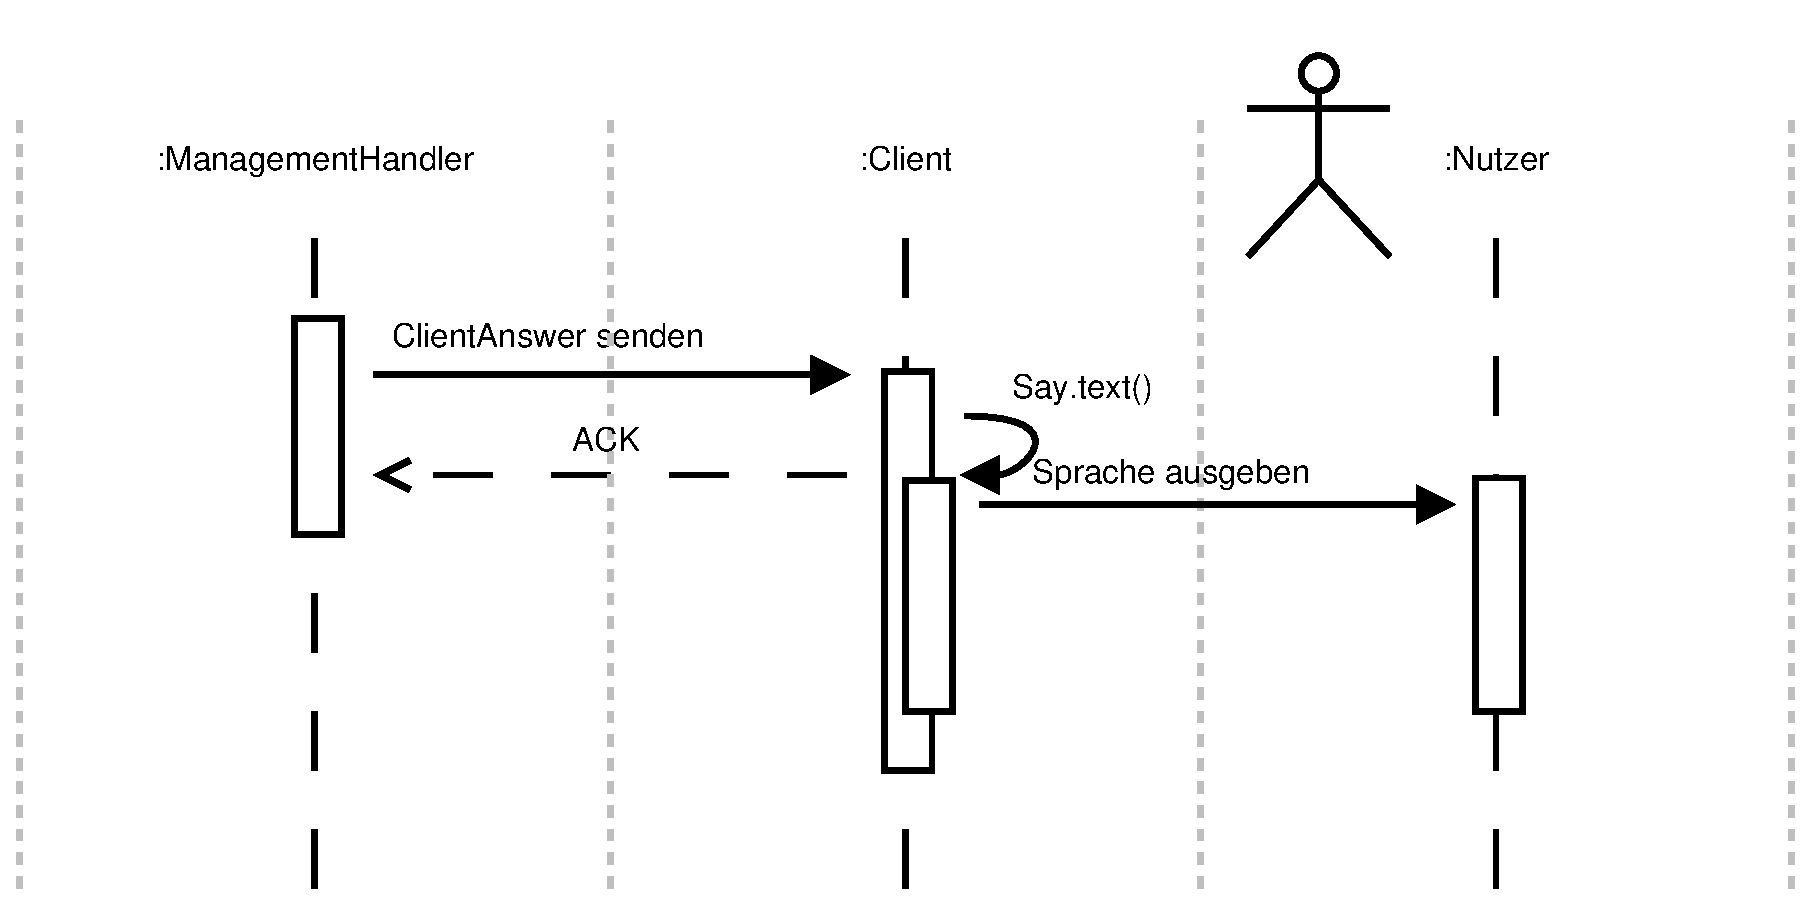
\includegraphics[width=.8\textwidth]{Systementwurf/02_produktfunktionsanalyse/f100}
\caption{Sequenzdiagramm \textit{\ref{F10} Sprachausgabe} \label{sd10}}
\end{figure}

\section{Analyse von Funktionalität \ref{F11}: Spracheingabe}

Um Anweisungen an \NewsGenie zu geben muss der Benutzer die Möglichkeit haben,
in natürlicher Sprache gesprochene Befehle einzugeben. Dazu betätigt er den
Aufnahmeknopf am \textit{Client}, woraufhin er ein visuelles Signal erhält und
die Aufnahme gestartet wird. Nun spricht der Benutzer seine Anweisung an \NewsGenie in das
Mikrofon. Sobald Stille eintritt, wird dies erkannt und die Anweisung als
Flac-Datei gespeichert. Dies wird in Abb.~\ref{sd11} dargestellt.

\begin{figure}[h]
\centering
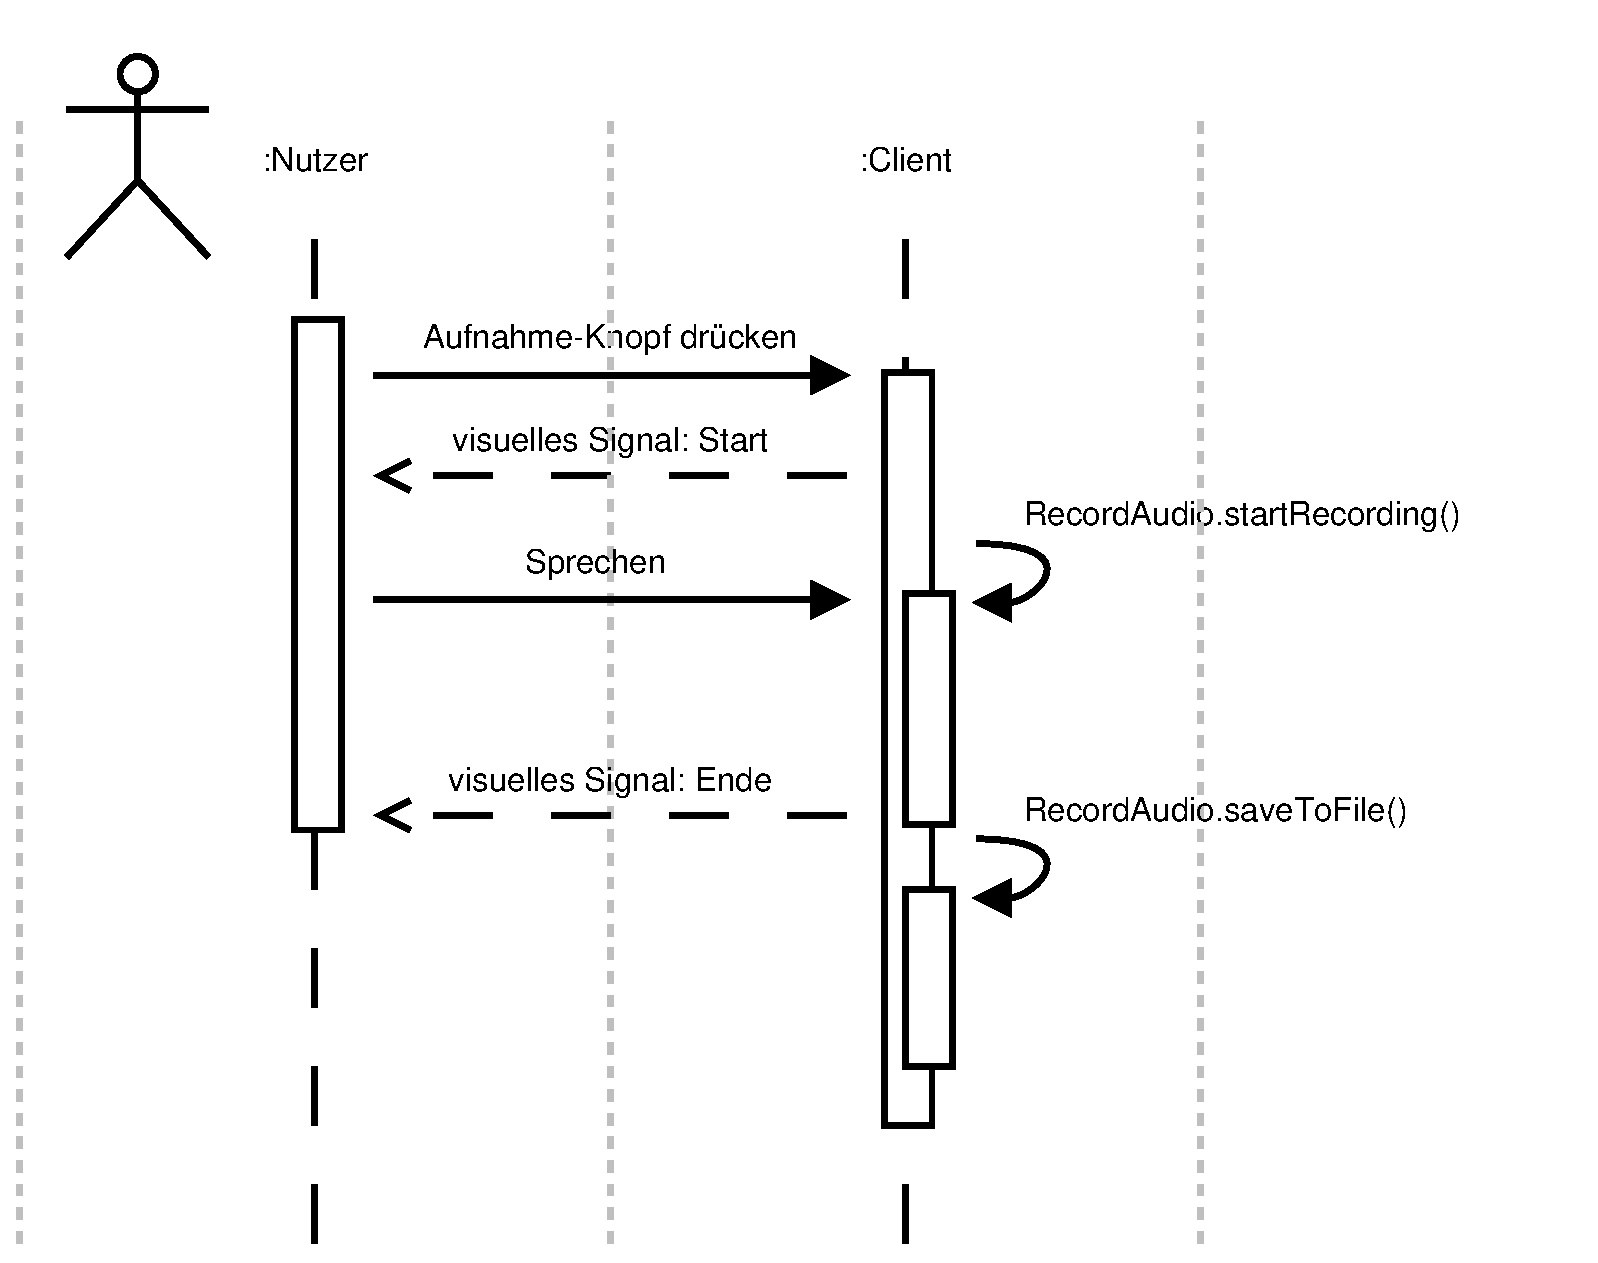
\includegraphics[width=.7\textwidth]{Systementwurf/02_produktfunktionsanalyse/f110}
\caption{Sequenzdiagramm \textit{\ref{F11} Spracheingabe} \label{sd11}}
\end{figure}

\FloatBarrier

\section{Analyse von Funktionalität \ref{F12}: Umwandlung von Sprache in Text}

Liegt beim \textit{Client} nach Ausführung der Funktion \ref{F11} eine
Flac-Datei zur Analyse vor, wird diese wie in Abb.~\ref{sd12} dargestellt vom
\textit{Client} an die \textit{GoogleSpeech API} gesendet. Nach Analyse der
Datei erhält der \textit{Client} ein \textit{GoogleResponse}-Objekt zurück.
Daraus wird anschließend der Text der Spracheingabe als String extrahiert.

\begin{figure}[h]
\centering
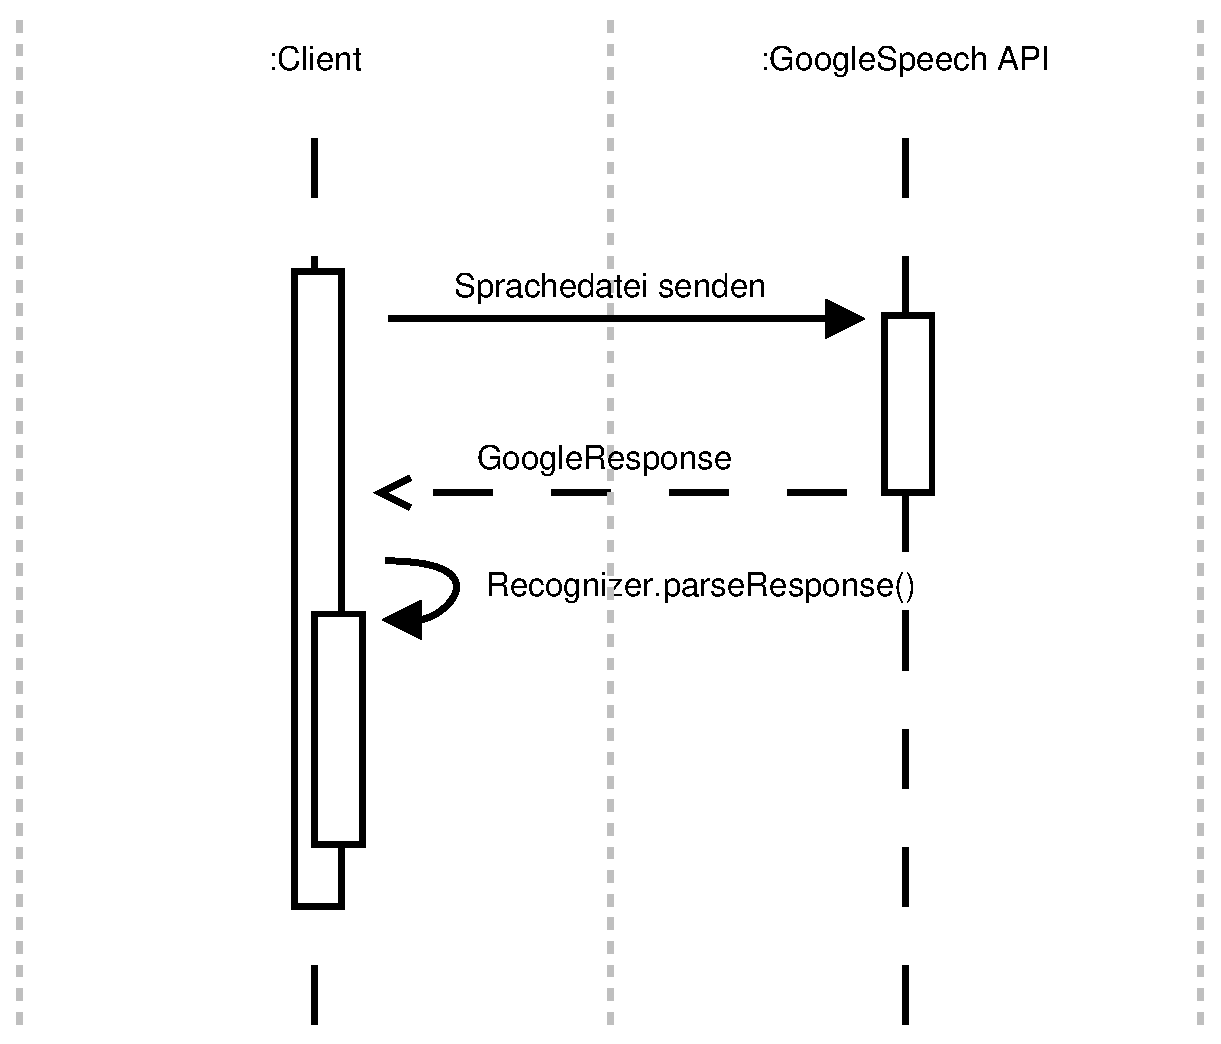
\includegraphics[width=.5\textwidth]{Systementwurf/02_produktfunktionsanalyse/f120}
\caption{Sequenzdiagramm \textit{\ref{F12} Umwandlung von Sprache in Text}
\label{sd12}}
\end{figure}


\section{Analyse von Funktionalität \ref{F13}: Umwandlung von Text in Sprache}

Die Umwandlung von Text in Sprache wird auf dem \textit{Client} mithilfe der
Software \textit{pico2wave} realisiert. Empfängt der Client ein
\textit{ClientAnswer}-Objekt vom \textit{ManagementHandler}, wie in Abb.
\ref{sd13}, wird diese über einen Systemaufruf in der Funktion
\textit{Say.text()} in eine Wave-Datei umgewandelt.

\begin{figure}[h]
\centering
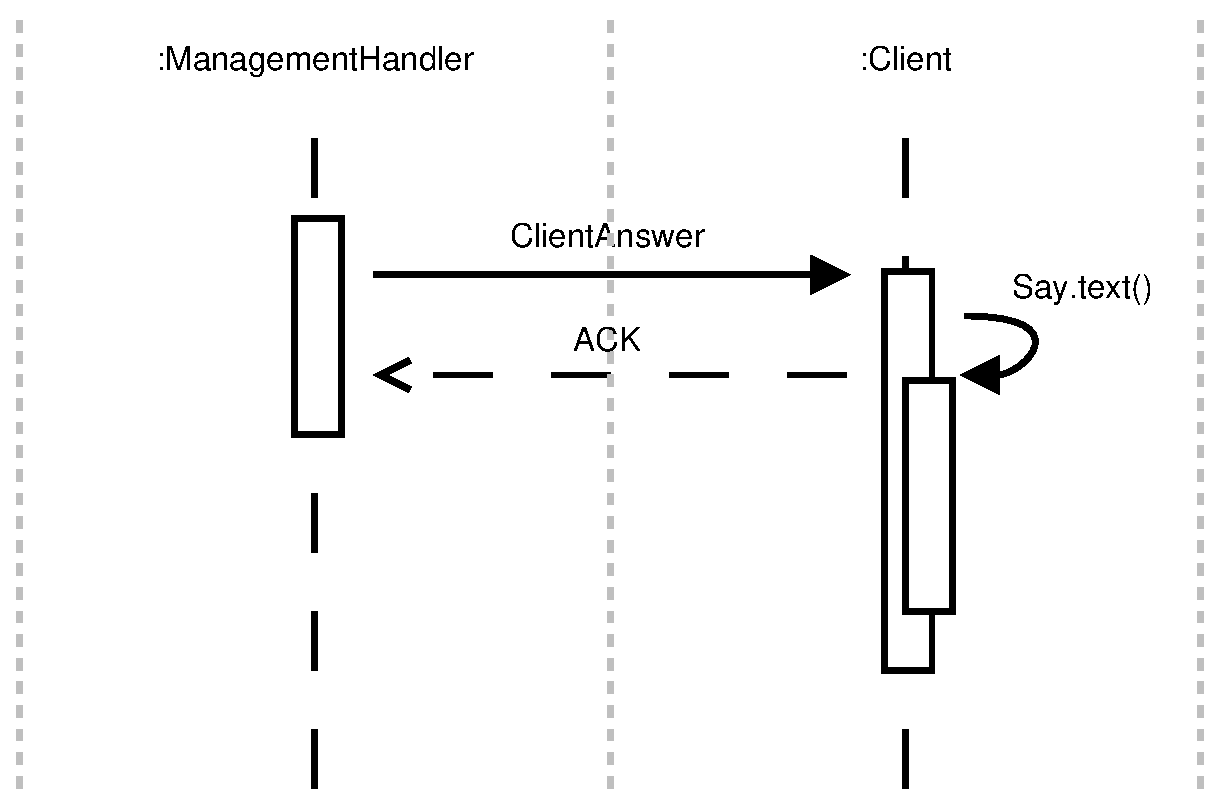
\includegraphics[width=.5\textwidth]{Systementwurf/02_produktfunktionsanalyse/f130}
\caption{Sequenzdiagramm \textit{\ref{F13} Umwandlung von Sprache in Text}
\label{sd13}}
\end{figure}

\FloatBarrier

\section{Analyse von Funktionalität \ref{F20}: Anfrage stellen}

An der Funktion \textit{Anfrage stellen} sind die Komponenten \textit{Client}
und
\textit{GoogleSpeechAPI} sowie auf dem Server \textit{ManagementHandler},
\textit{QueryHandler} und \textit{DatabaseHandler} beteiligt. Die Teilfunktionen
\ref{F10}, \ref{F11}, \ref{F12}, \ref{F13} werden als Teile dieser Funktion
aufgerufen und im entsprechenden Sequenzdiagramm Abb.~\ref{sd20} nur vereinfacht
dargestellt.

Zuerst wird vom \textit{Nutzer} eine Sprachaufzeichnung \ref{F11} auf dem Client
gestartet, welcher daraufhin die aufgezeichnete Sprachdatei mithilfe von
\ref{F12} in Text umwandelt. Vom \textit{Client} wird nun ein
\textit{ClientQuery}-Objekt generiert und über den \textit{ManagementHandler}
dem \textit{Query-Processor} auf dem Server übergeben. Dieser analysiert die
Anfrage und startet eine entsprechende Datenbanksuche durch Übergabe eines
\textit{SearchRequest}-Objektes an den \textit{DatenbankHandler}. Das
Suchergebnis wird als \textit{SearchAnswer}-Objekt an den \textit{QueryProcessor}
zurückgegeben, in eine Textantwort aus zusammenhängenden Sätzen umgewandelt und
als \textit{ClientAnswer}-Objekt über den \textit{ManagementHandler} an den
\textit{Client} zurückgegeben. Dieser wandelt die Antwort unter Zuhilfenahme von
\ref{F13} und \ref{F10} in eine Sprachausgabe um und spielt diese ab.

\begin{figure}[h]
\centering
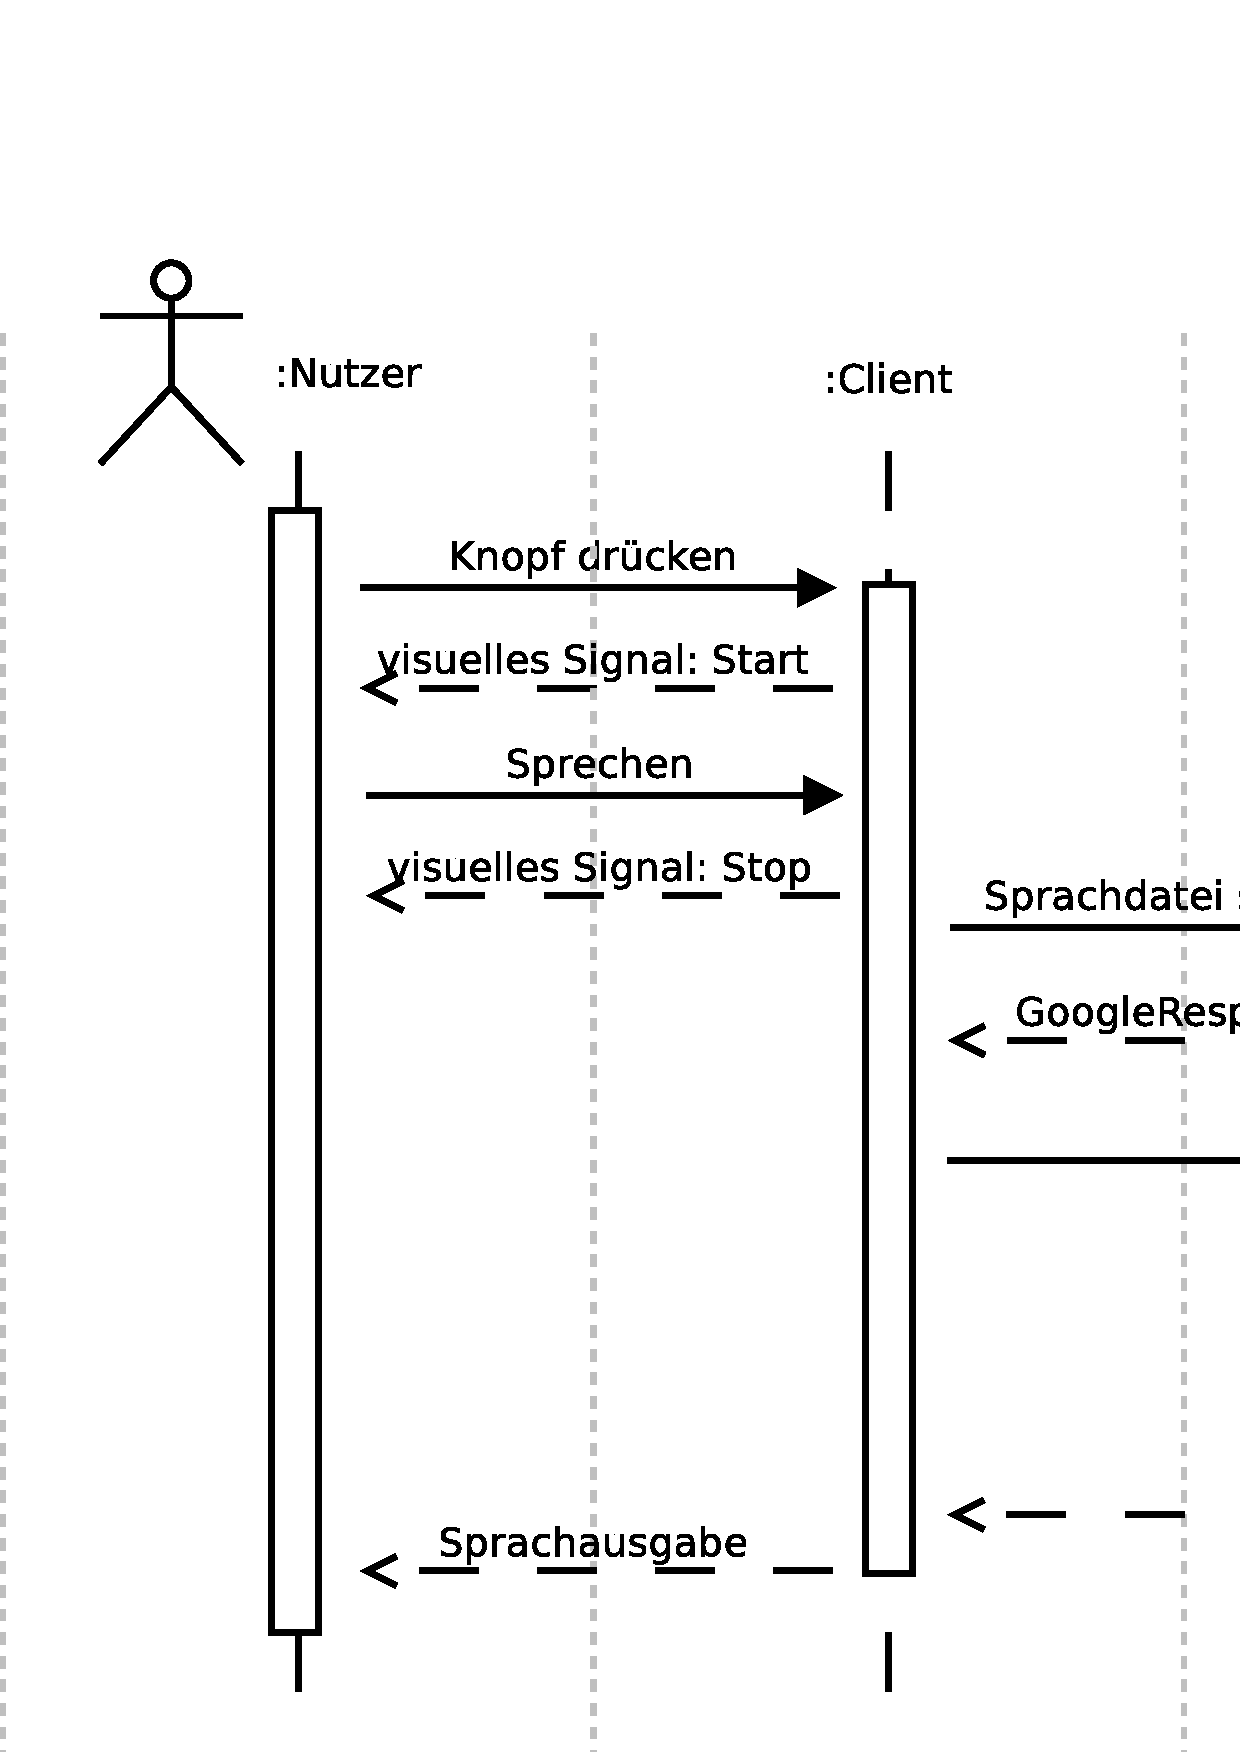
\includegraphics[width=1\textheight, angle=90]{Systementwurf/02_produktfunktionsanalyse/f200}
\caption{Sequenzdiagramm \textit{\ref{F20} Anfrage stellen}
\label{sd20}}
\end{figure}


\section{Analyse von Funktionalität \ref{F30}: Client Login}

Um Anfragen an \NewsGenie stellen zu können, muss ein Benutzer sich erst am
\textit{Client} identifizieren. Da keine sensiblen Informationen über den Client
abgerufen werden können und eine Passworteingabe per Sprache unpraktikabel ist,
erfolgt dies durch Nennung des Benutzernamens. Dabei kommen  \ref{F11} für die
Sprachaufzeichnung am \textit{Client} und \ref{F12} für die anschließende
Umwandlung der Wave-Datei in einen String zum Einsatz. Wie in Abb.~\ref{sd30}
dargestellt wird anschließend vom \textit{Client} ein
\textit{ClientQuery}-Objekt an den \textit{ManagementHandler} auf dem Server
übertragen. Dieser reicht es zur Analyse an den \textit{QueryProcessor} weiter,
der anhand von Schlüsselwörtern erkennt, dass es sich um eine Login-Anfrage
handelt. Er liefert ein \textit{ClientLogin}-Objekt an den
\textit{ManagementHandler} zurück. Dieser veranlasst nun, dass ein
\textit{ClientLoginRequest}-Objekt an den \textit{DatabaseHandler} gesandt wird.
Jetzt wird überprüft ob der entsprechende Benutzer in der Datenbank vorhanden
ist und ein \textit{ClientLoginAnswer}-Objekt zurückgeschickt, dass den Benutzer
(sofern vorhanden) enthält.

Der \textit{ManagementHandler} veranlasst nun durch Senden des
\textit{ClientLogin}-Objektes eine entsprechende Sprachnachricht am Client,
wobei wiederum \ref{F13} und \ref{F10} genutzt werden.

\begin{figure}[h]
\centering
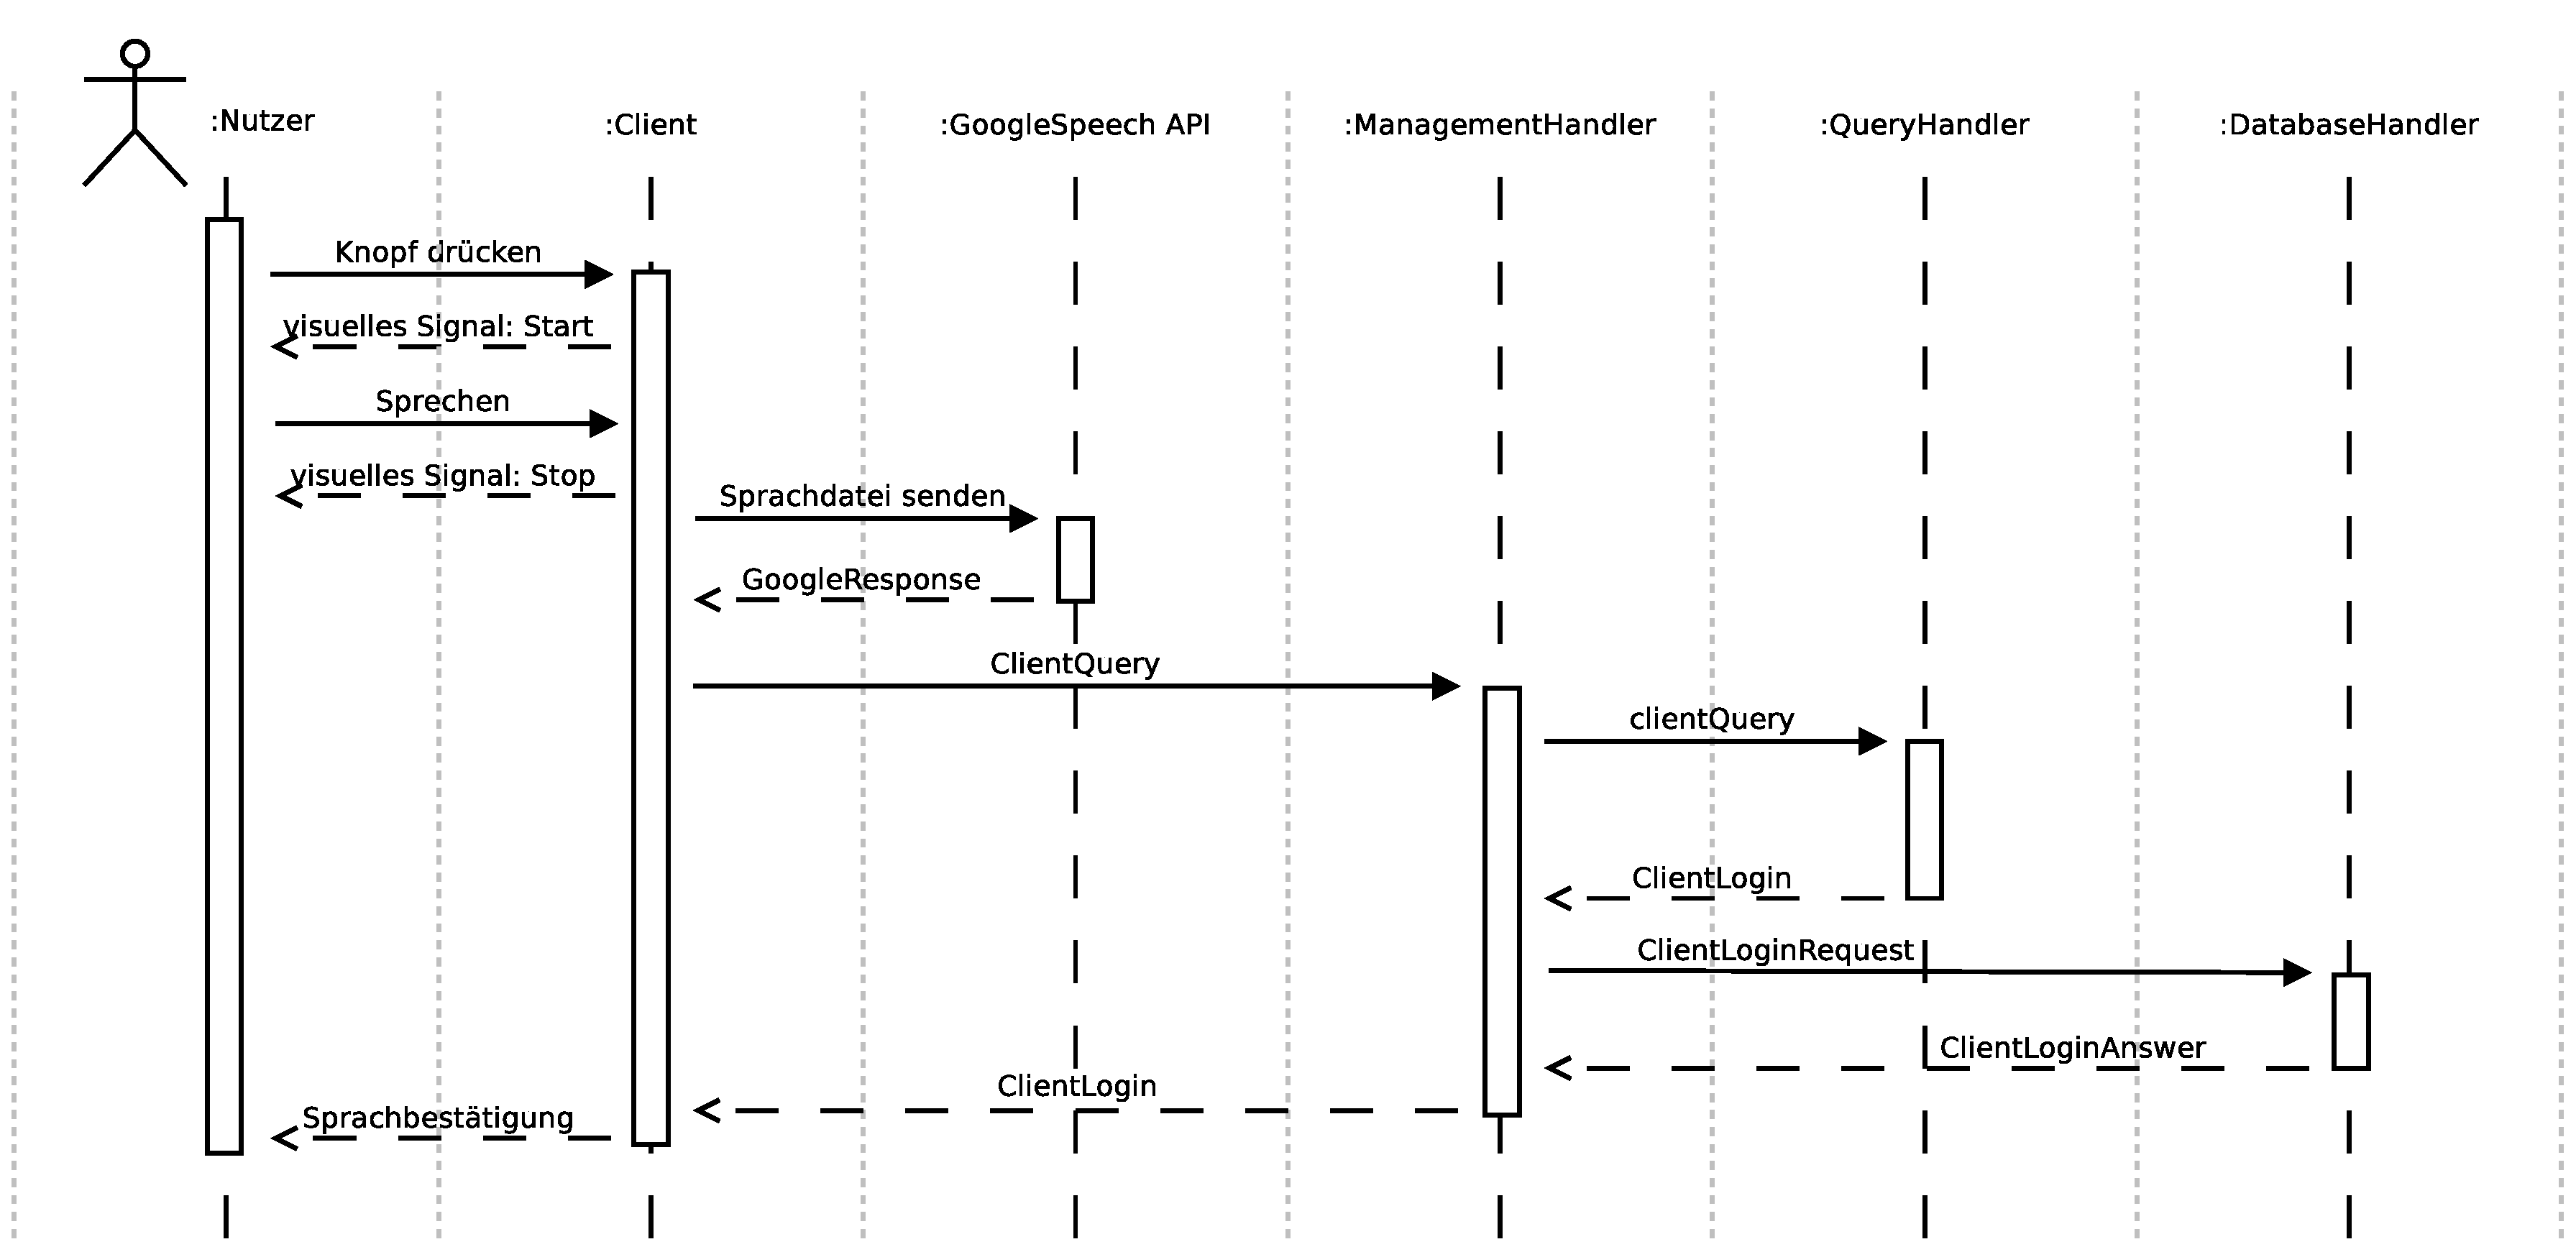
\includegraphics[width=1\textheight, angle=90]{Systementwurf/02_produktfunktionsanalyse/f300}
\caption{Sequenzdiagramm \textit{\ref{F30} Client Login}
\label{sd30}}
\end{figure}

\FloatBarrier

\section{Analyse von Funktionalität \ref{F31}: Client Logout}

Ist ein Benutzer am \textit{Client} angemeldet, wird durch einen Timer die Zeit
seit der letzten Aktion des Benutzers festgehalten. Wird dabei ein bestimmter
Schwellenwert überschritten (etwa 5 Minuten), so wird der Benutzer automatisch
am Client abgemeldet. Eine Nachricht an den Server ist dafür nicht notwendig, da
dieser nicht speichert, welcher Benutzer an welchem Client angemeldet ist.
Dies wird im Sequenzdiagramm in Abb.~\ref{sd31} dargestellt.

\begin{figure}[h]
\centering
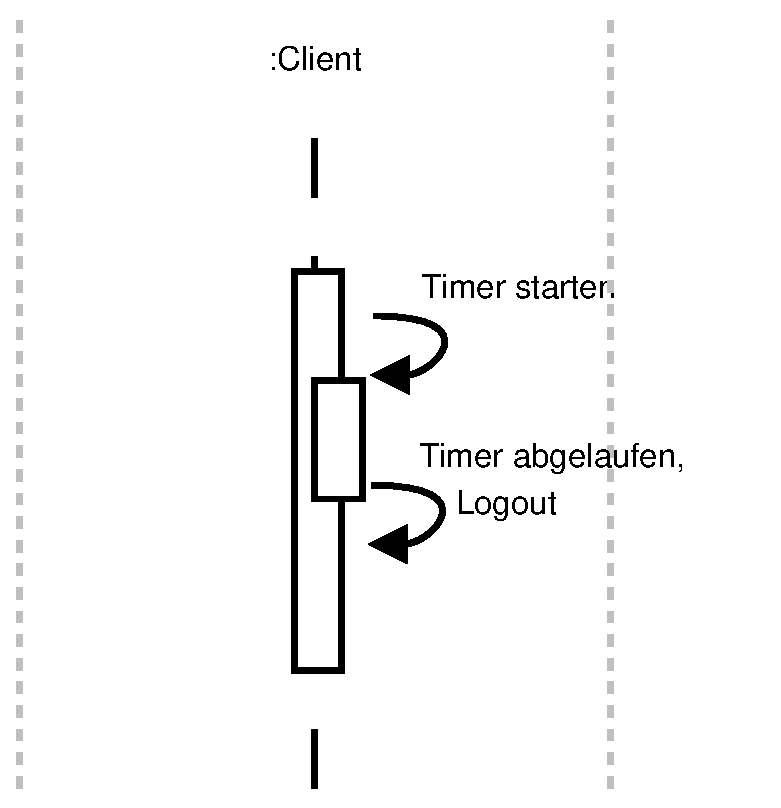
\includegraphics[width=.3\textwidth]{Systementwurf/02_produktfunktionsanalyse/f310}
\caption{Sequenzdiagramm \textit{\ref{F31} Client Logout}
\label{sd31}}
\end{figure}


\section{Analyse von Funktionalität \ref{F40}: News-Crawling}

In Abb.~\ref{sd40} wird der kontinuierlich stattfindende Abruf neuer Nachricht
aus den gespeicherten RSS-Feeds der Benutzer dargestellt. Dabei wird die
Prozedur für jeden gespeicherten Feed in festgelegten Zeitabständen
durchgeführt. Der \textit{Crawler} fragt dabei die entsprechenden
\textit{RSS-Feeds} ab und prüft anschließend durch eine Abfrage beim
\textit{DatabaseHandler} ob die abgerufenen Artikel schon in die Datenbank
aufgenommen wurden. Anschließend trägt er die als neu identifizierten Artikel in
die Datenbank ein.

\begin{figure}[h]
\centering
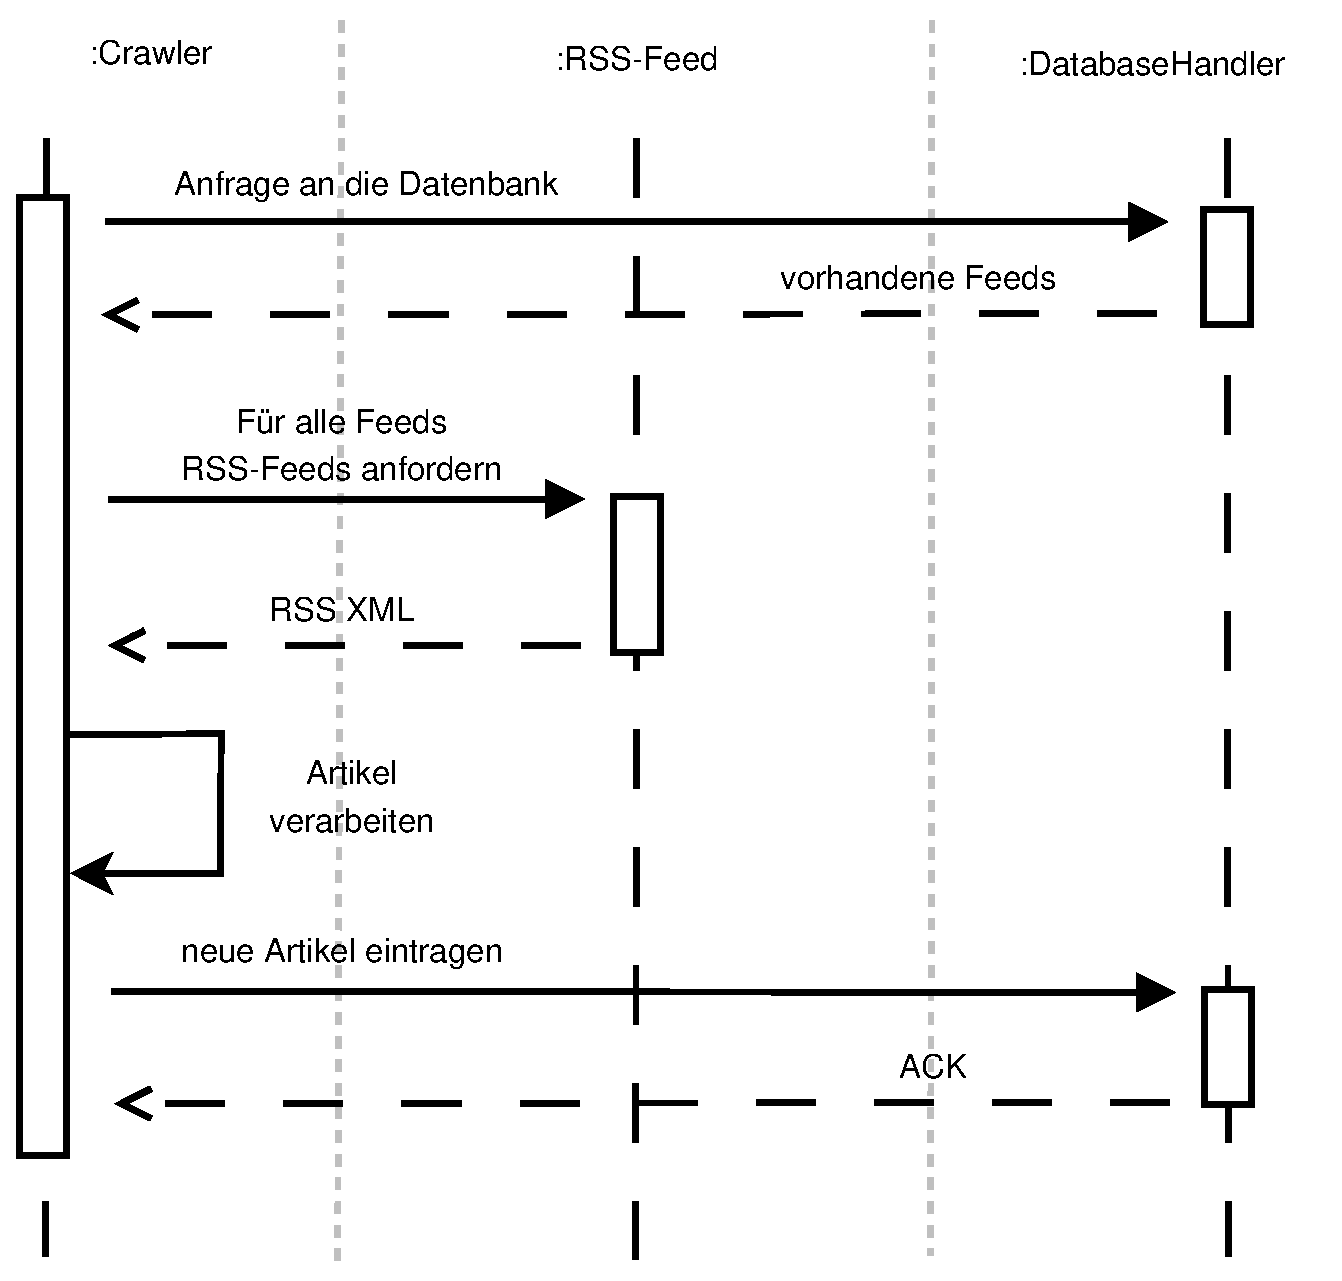
\includegraphics[width=.7\textwidth]{Systementwurf/02_produktfunktionsanalyse/f400}
\caption{Sequenzdiagramm \textit{\ref{F40} News-Crawling}
\label{sd40}}
\end{figure}

\FloatBarrier

\section{Analyse von Funktionalität \ref{F50}: Registrierung}

Die Registrierung als Benutzer von \NewsGenie ist notwendig um die Clients
nutzen zu können und eigene Feeds zu verwalten. Diese Registrierung erfolgt
hierbei nicht am \textit{Client}, sondern wird über ein \textit{WebInterface}
vorgenommen.

Der Benutzer füllt dazu das Registrierungsformular im \textit{WebInterface} aus,
welches anschließend die eingegebenen Daten wie Benutzername, Email und Passwort
an den \textit{WebHandler} auf dem Server überträgt. Dieser sendet wie in Abb.
\ref{sd50} gezeigt einen \textit{RegisterRequest} an den
\textit{DatabaseHandler} welcher mit einem \textit{RegisterAnswer}-Objekt an den 
\textit{WebHandler} zurückgibt. Dieser veranlasst die Ausgabe einer
Erfolgsmeldung vom \textit{WebInterface} an den Benutzer.

\begin{figure}[h]
\centering
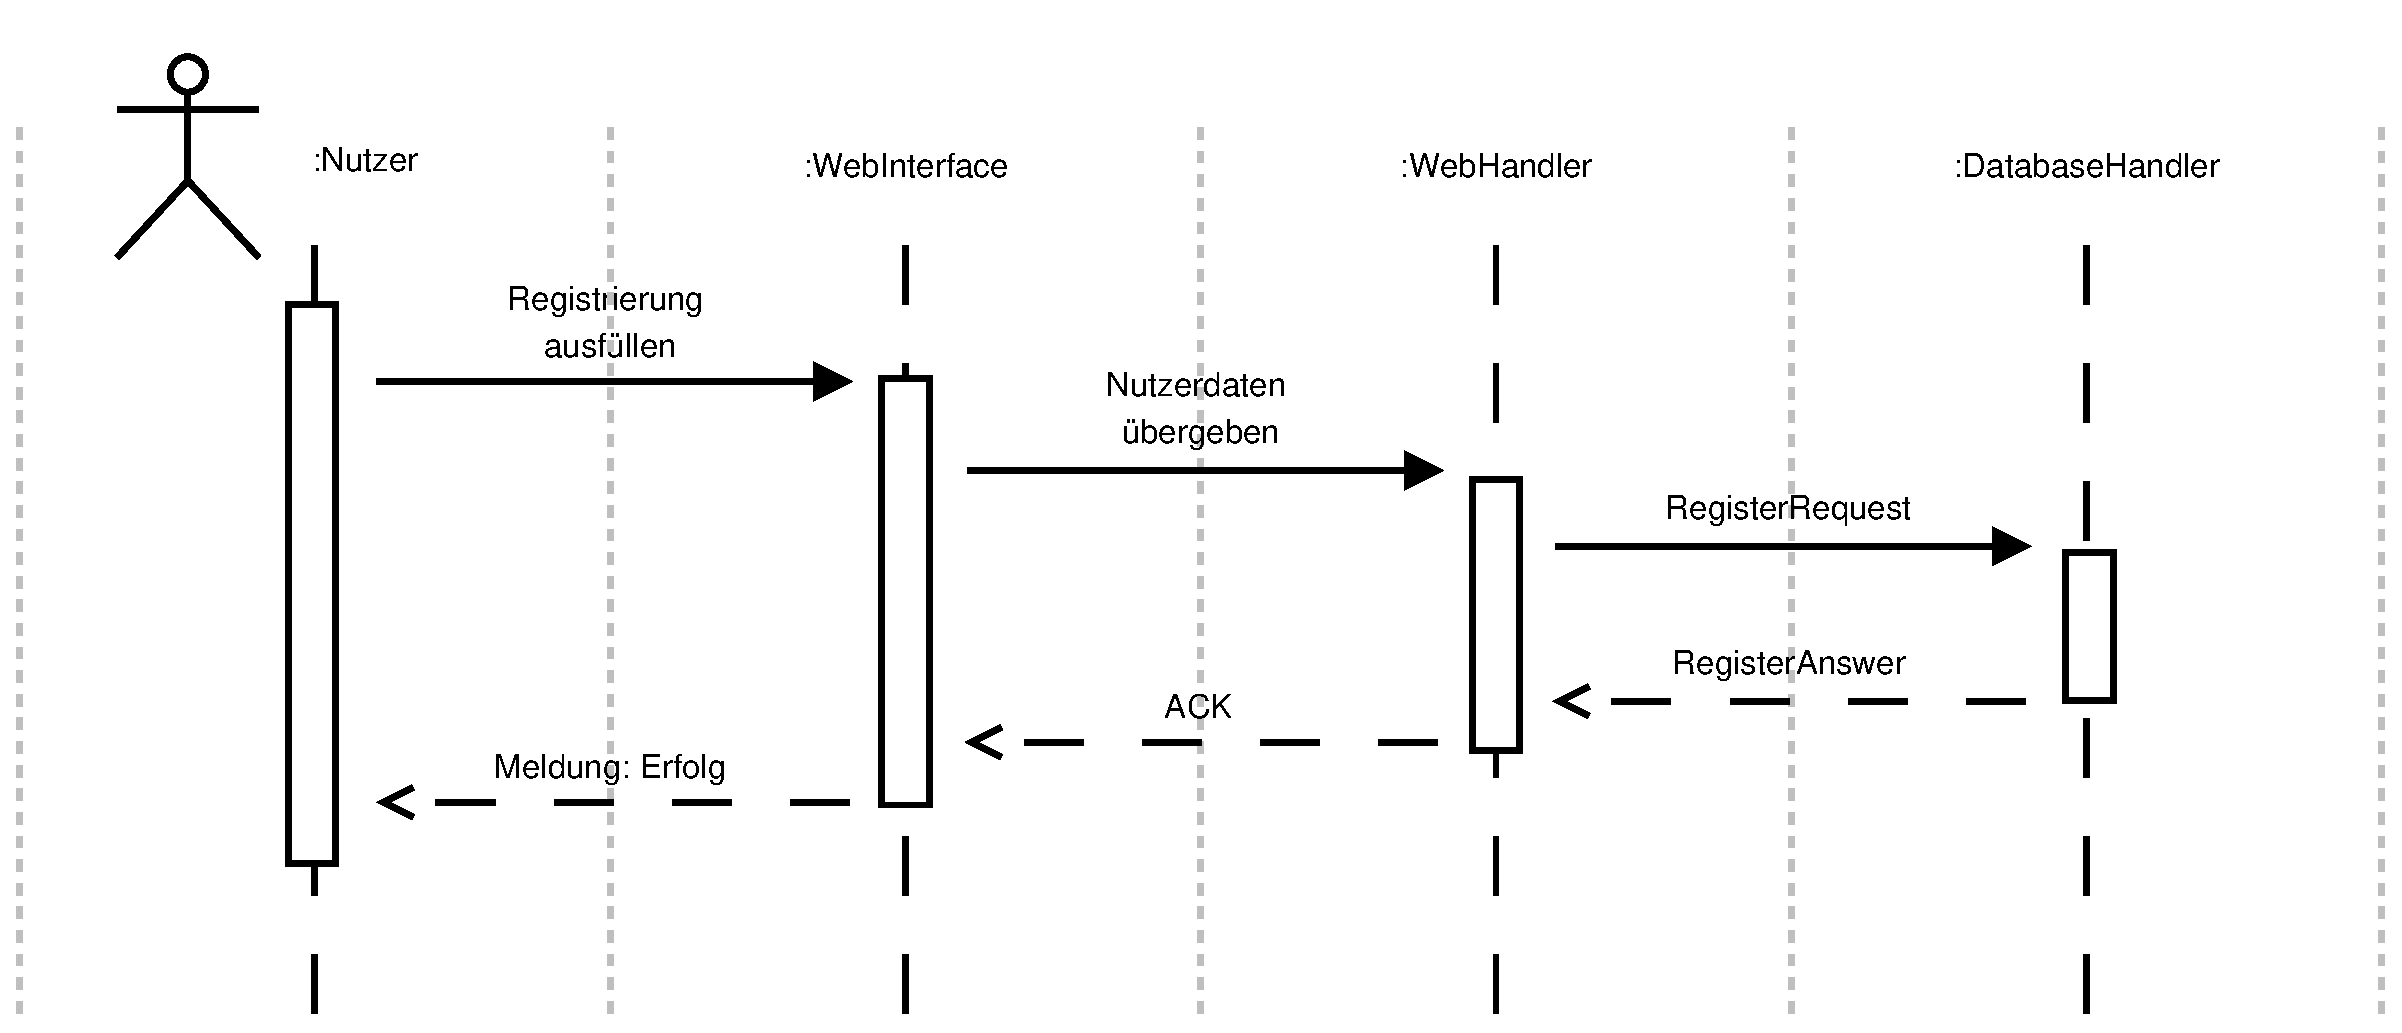
\includegraphics[width=1\textwidth]{Systementwurf/02_produktfunktionsanalyse/f500}
\caption{Sequenzdiagramm \textit{\ref{F50} Registrierung}
\label{sd50}}
\end{figure}


\section{Analyse von Funktionalität \ref{F60}: Webinterface-Login}

Um im \textit{WebInterface} Einstellungen vornehmen zu können, muss sich ein
Benutzer zuerst einloggen. In Abb.~\ref{sd60} sieht man, dass dazu vom Benutzer
das Login Formular im \textit{WebInterface} ausgefüllt wird und anschließend vom
\textit{WebHandler} der eingegebene Benutzername und das Passwort als
\textit{WebLoginRequest}-Objekt an den \textit{DatabaseHandler} geschickt werden
der durch zurücksenden eines \textit{WebLoginAnswer}-Objektes mitteilt, ob ein
entsprechender Benutzer in der Datenbank gefunden wurde. Das
\textit{WebInterface} wird in diesem Fall angewiesen, eine Erfolgsmeldung an den
Nutzer zu geben.

\begin{figure}[h]
\centering
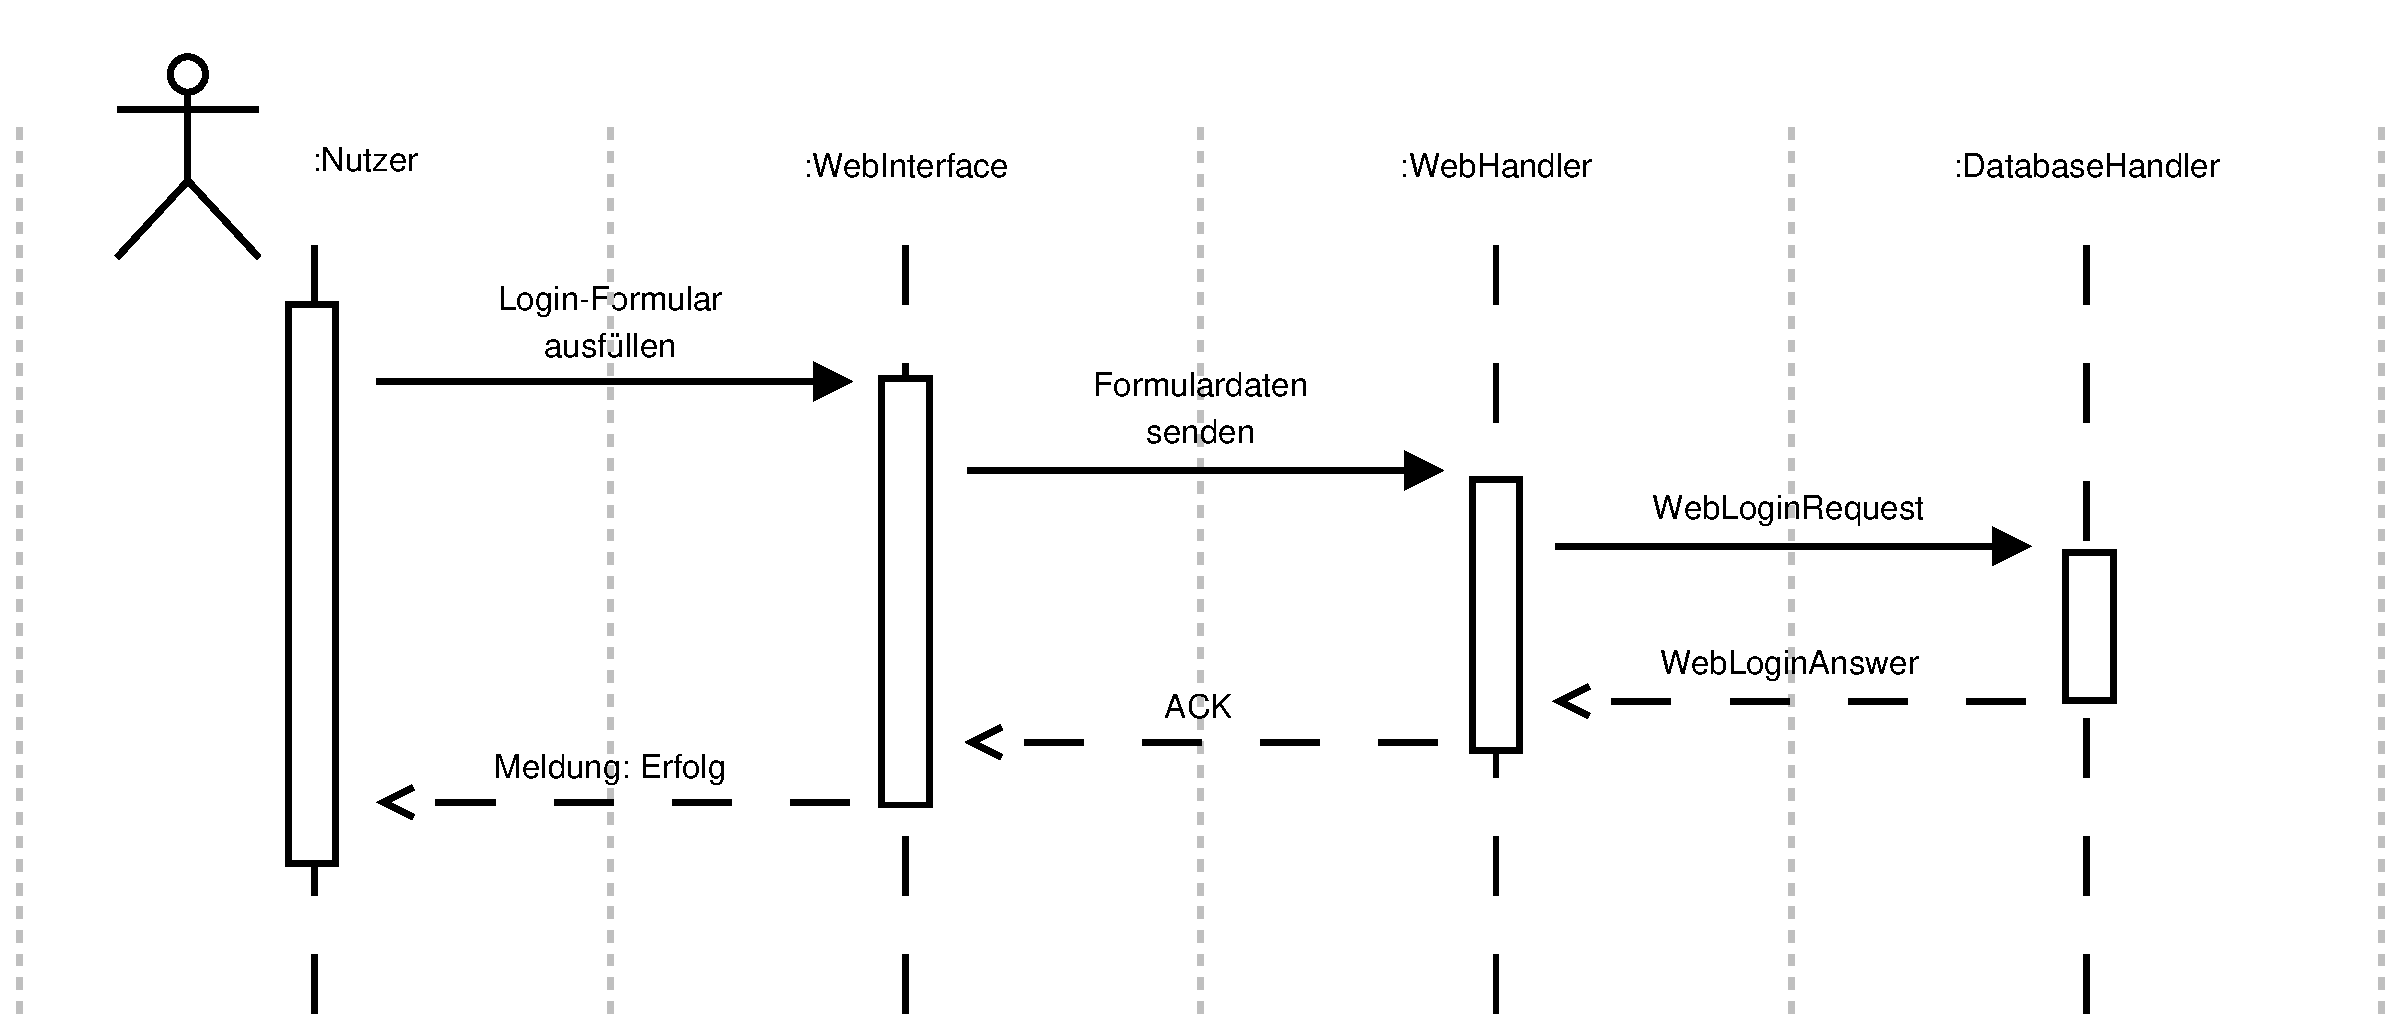
\includegraphics[width=1\textwidth]{Systementwurf/02_produktfunktionsanalyse/f600}
\caption{Sequenzdiagramm \textit{\ref{F60} Webinterface-Login}
\label{sd60}}
\end{figure}


\section{Analyse von Funktionalität \ref{F61}: Webinterface-Logout}

Ist ein Benutzer im \textit{WebInterface} eingeloggt und betätigt wie in Abb.~\ref{sd61} gezeigt den Logout-Button sendet das \textit{WebInterface} einen
\textit{LogoutRequest} an den \textit{WebHandler}. Dieser beendet die Session
des Benutzers und weist das \textit{WebInterface} an, eine Erfolgsmeldung
auszugeben.

\begin{figure}[h]
\centering
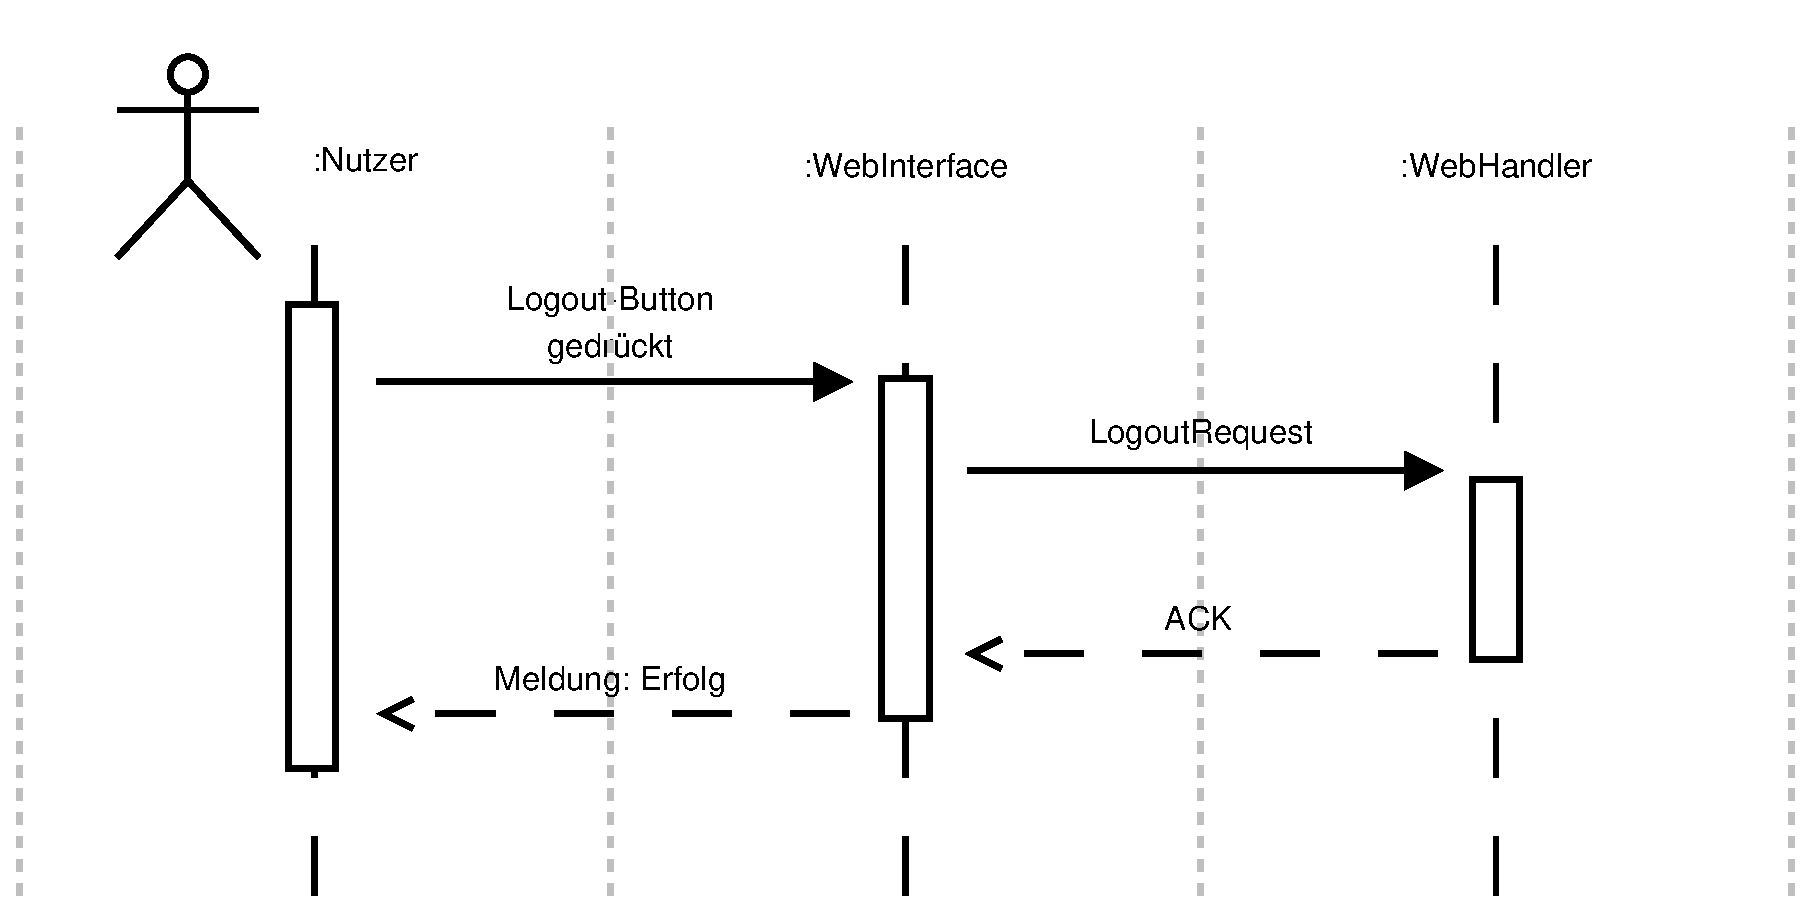
\includegraphics[width=.8\textwidth]{Systementwurf/02_produktfunktionsanalyse/f610}
\caption{Sequenzdiagramm \textit{\ref{F61} Webinterface-Logout}
\label{sd61}}
\end{figure}

\FloatBarrier

\section{Analyse von Funktionalität \ref{F70}: Feed-Liste anzeigen}

Über diese Funktion hat der Benutzer die Möglichkeit, sich eine Übersicht über seine
RSS-Feeds zu verschaffen und die weiteren Funktionen wie \ref{F71} und \ref{F72}
aufzurufen. In Abb.~\ref{sd70} wird gezeigt, dass der Nutzer durch Aufruf eines
Links im \textit{WebInterface} die Feedliste beim \textit{WebHandler} anfordert.
Dieser fragt durch Übergabe eines \textit{UserFeedRequest}-Objektes an den
\textit{DatabaseHandler} die Feeds des Users ab und erhält ein
\textit{UserFeedAnswer}-Objekt zurück, welches die Feeds des Benutzers enthält.
Der \textit{WebHandler} gibt nun über das \textit{WebInterface} die Feedliste an
den Benutzer aus.

\begin{figure}[h]
\centering
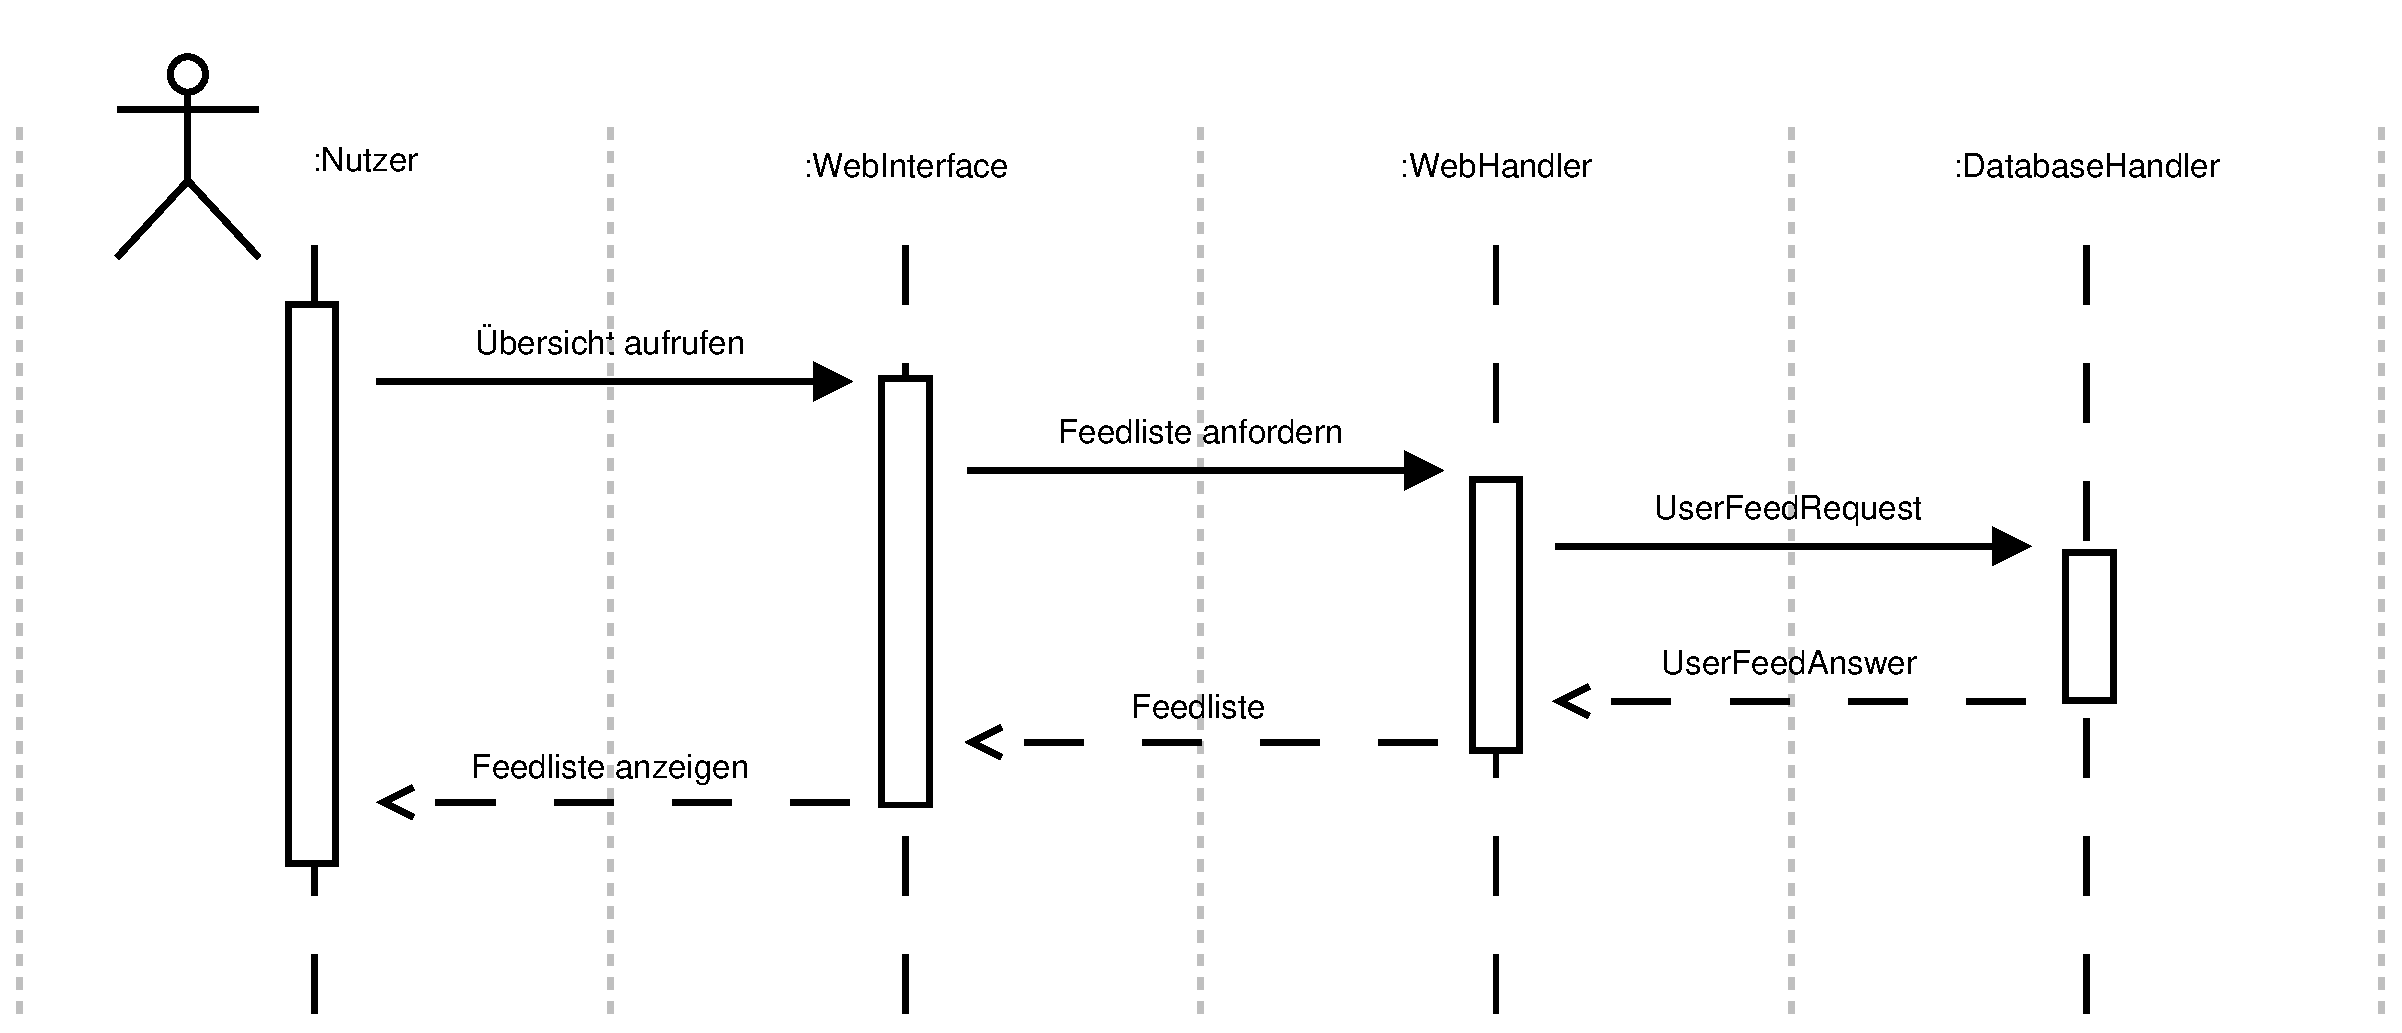
\includegraphics[width=1\textwidth]{Systementwurf/02_produktfunktionsanalyse/f700}
\caption{Sequenzdiagramm \textit{\ref{F70} Feed-Liste anzeigen}
\label{sd70}}
\end{figure}

\FloatBarrier

\section{Analyse von Funktionalität \ref{F71}: Feed hinzufügen}

Ist der Benutzer im \textit{WebInterface} eingeloggt hat er die Möglichkeit neue
RSS-Feeds zu seinen Nachrichtenquellen hinzuzufügen. Dazu gibt er im
\textit{WebInterface} die URL des Feeds an. Durch das Absenden des Formulares
wird vom \textit{WebInterface} die URL an den \textit{WebHandler} übergeben.
Dieser sendet ein \textit{AddFeedRequest}-Objekt an den
\textit{DatabaseHandler}. Als Bestätigung erhält er, wie in Abb.~\ref{sd71}
gezeigt, ein \textit{AddFeedAnswer}-Objekt zurück.

\begin{figure}[h]
\centering
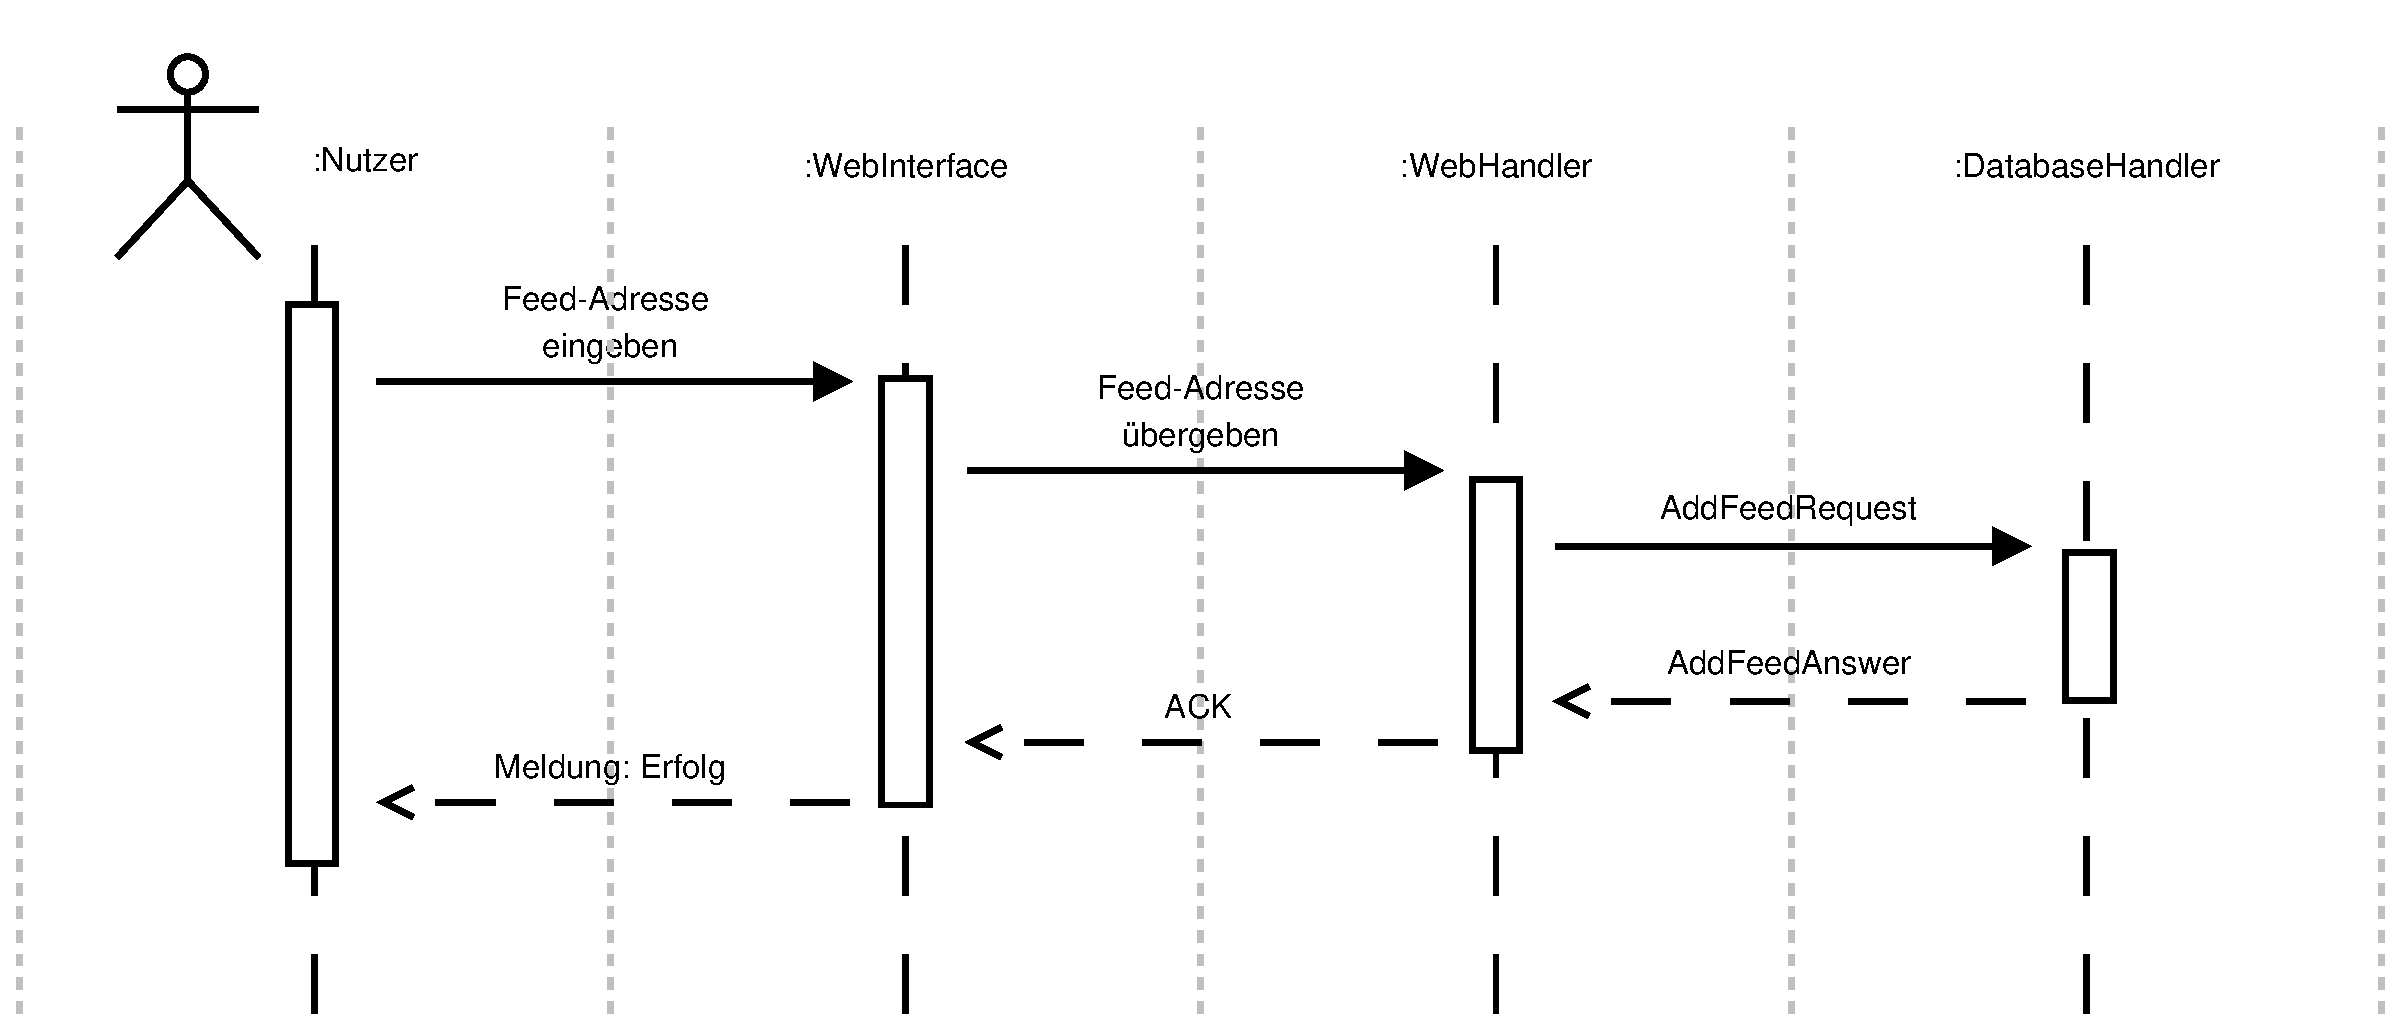
\includegraphics[width=1\textwidth]{Systementwurf/02_produktfunktionsanalyse/f710}
\caption{Sequenzdiagramm \textit{\ref{F71} Feed hinzufügen}
\label{sd71}}
\end{figure}


\section{Analyse von Funktionalität \ref{F72}: Feed entfernen}

Um Nachrichtenquellen zu entfernen muss der Benutzer im \textit{WebInterface}
eingeloggt sein. In der von \ref{F70} generierten Feed-Liste befindet sich neben
jedem Feed ein Button zum Löschen des Feeds. In Abb.~\ref{sd72} wird gezeigt,
dass durch Betätigen dieses Links im \textit{WebInterface} eine
Löschaufforderung an den \textit{WebHandler} gesendet wird. Dieser übergibt ein
\textit{RemoveFeedRequest}-Objekt an den \textit{DatabaseHandler}. Dieser
quittiert die Löschung mit einem \textit{RemoveFeedAnswer}-Objekt, was den
\textit{WebHandler} dazu veranlasst vom \textit{WebInterface} eine
Erfolgsmeldung an den Benutzer ausgeben zu lassen.

\begin{figure}[h]
\centering
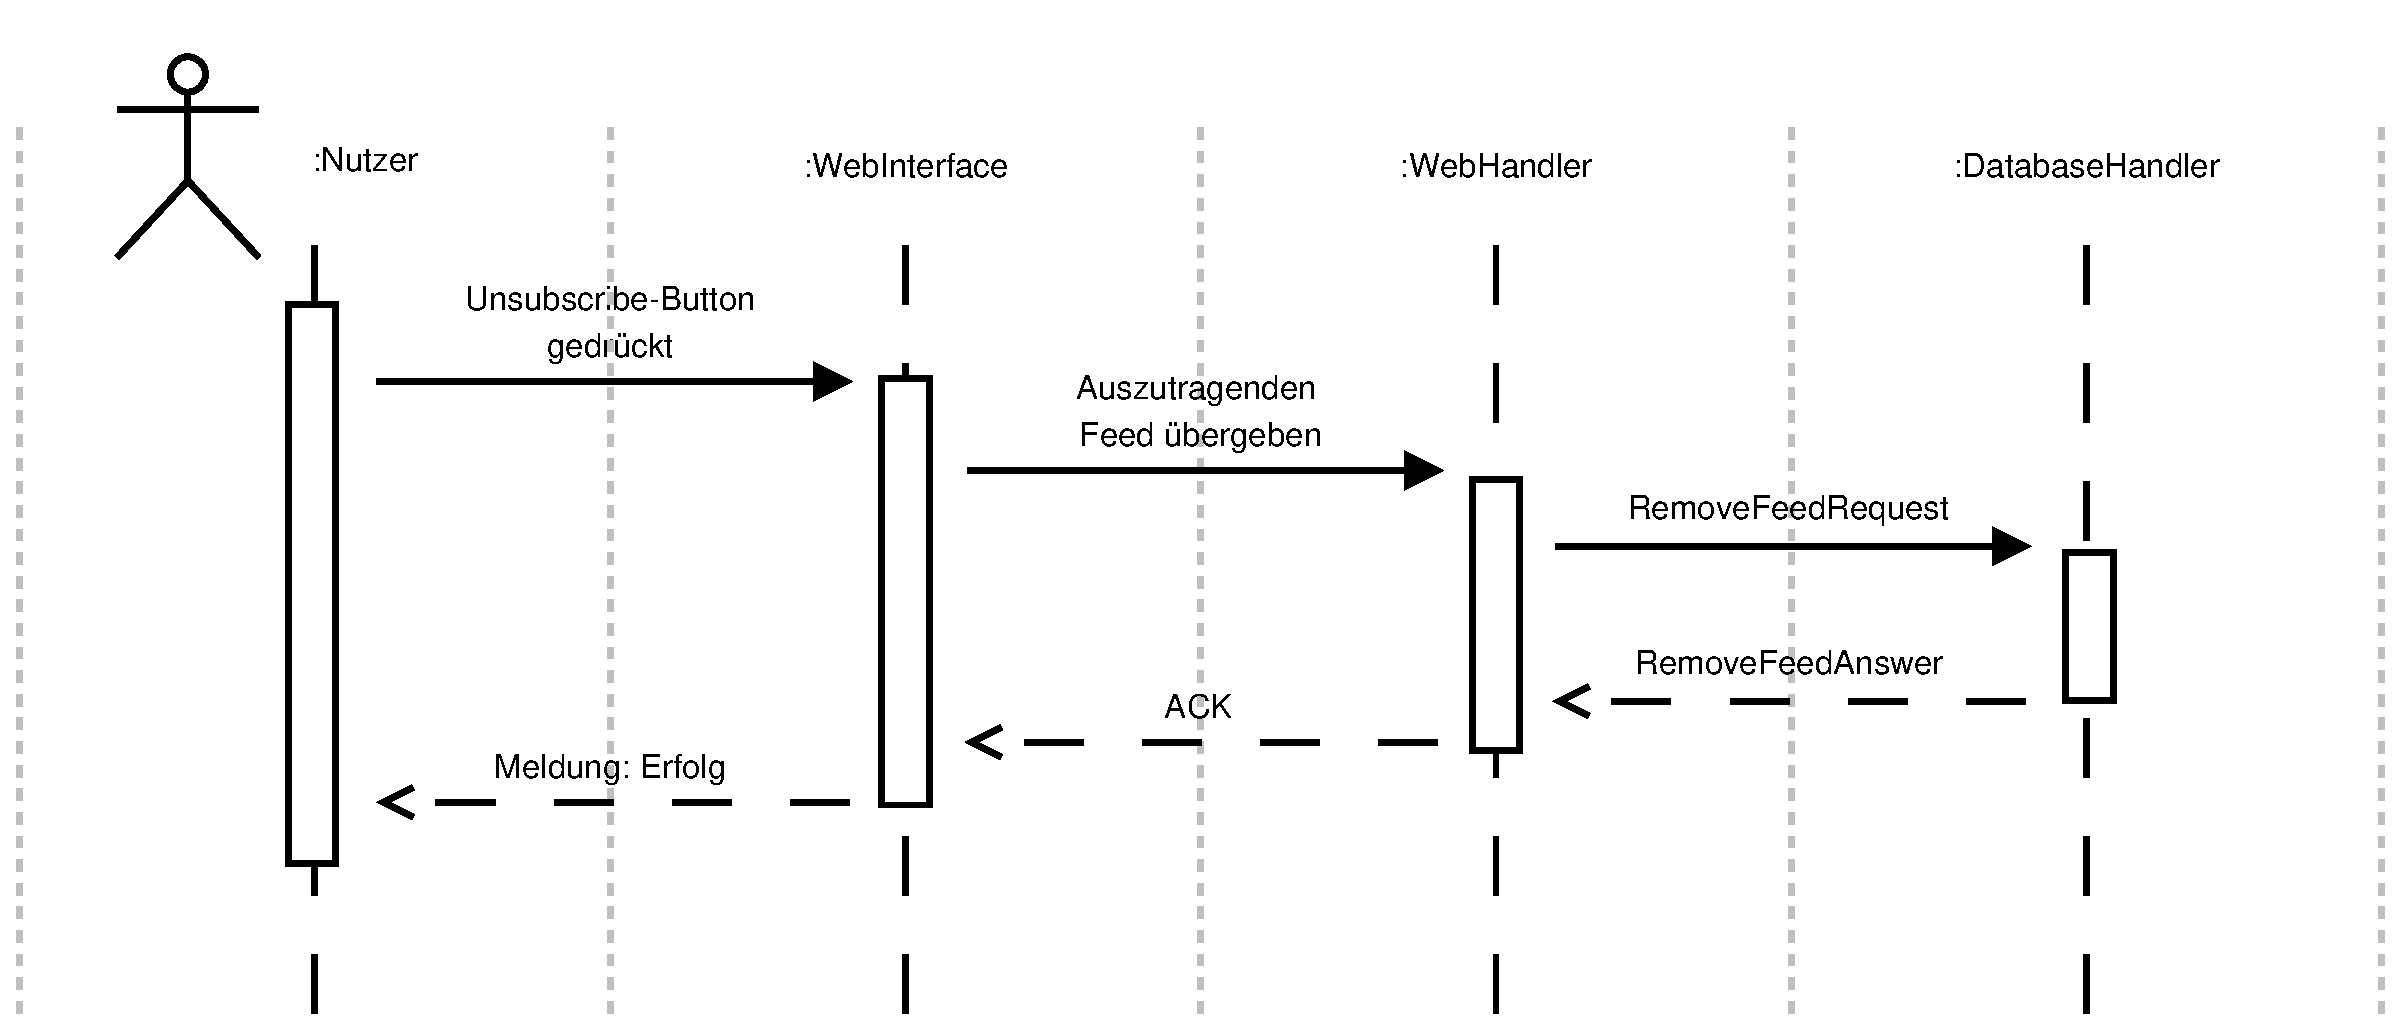
\includegraphics[width=1\textwidth]{Systementwurf/02_produktfunktionsanalyse/f720}
\caption{Sequenzdiagramm \textit{\ref{F72} Feed entfernen}
\label{sd72}}
\end{figure}

\FloatBarrier

\section{Analyse von Funktionalität \ref{F80}: Passwort ändern}

Im \textit{WebInterface} hat der Benutzer auch die Möglichkeit, sein Passwort zu
ändern. Dazu sendet er, in eingeloggtem Zustand, ein Formular mit dem alten und
dem neuen Passwort (dies in doppelter Ausführung) ab. Das \textit{WebInterface}
überträgt diese Informationen nun an den \textit{WebHandler}, welcher ein
\textit{ChangePasswordRequest}-Objekt an den \textit{DatabaseHandler} sendet.
Vom \textit{DatabaseHandler} erhält der \textit{WebHandler} nun ein
\textit{ChangePasswordAnswer}-Objekt zurück und weist das \textit{WebInterface}
an, eine Erfolgsmeldung an den Nutzer zu geben, wie in Abb.~\ref{sd80}
dargestellt.

\begin{figure}[h]
\centering
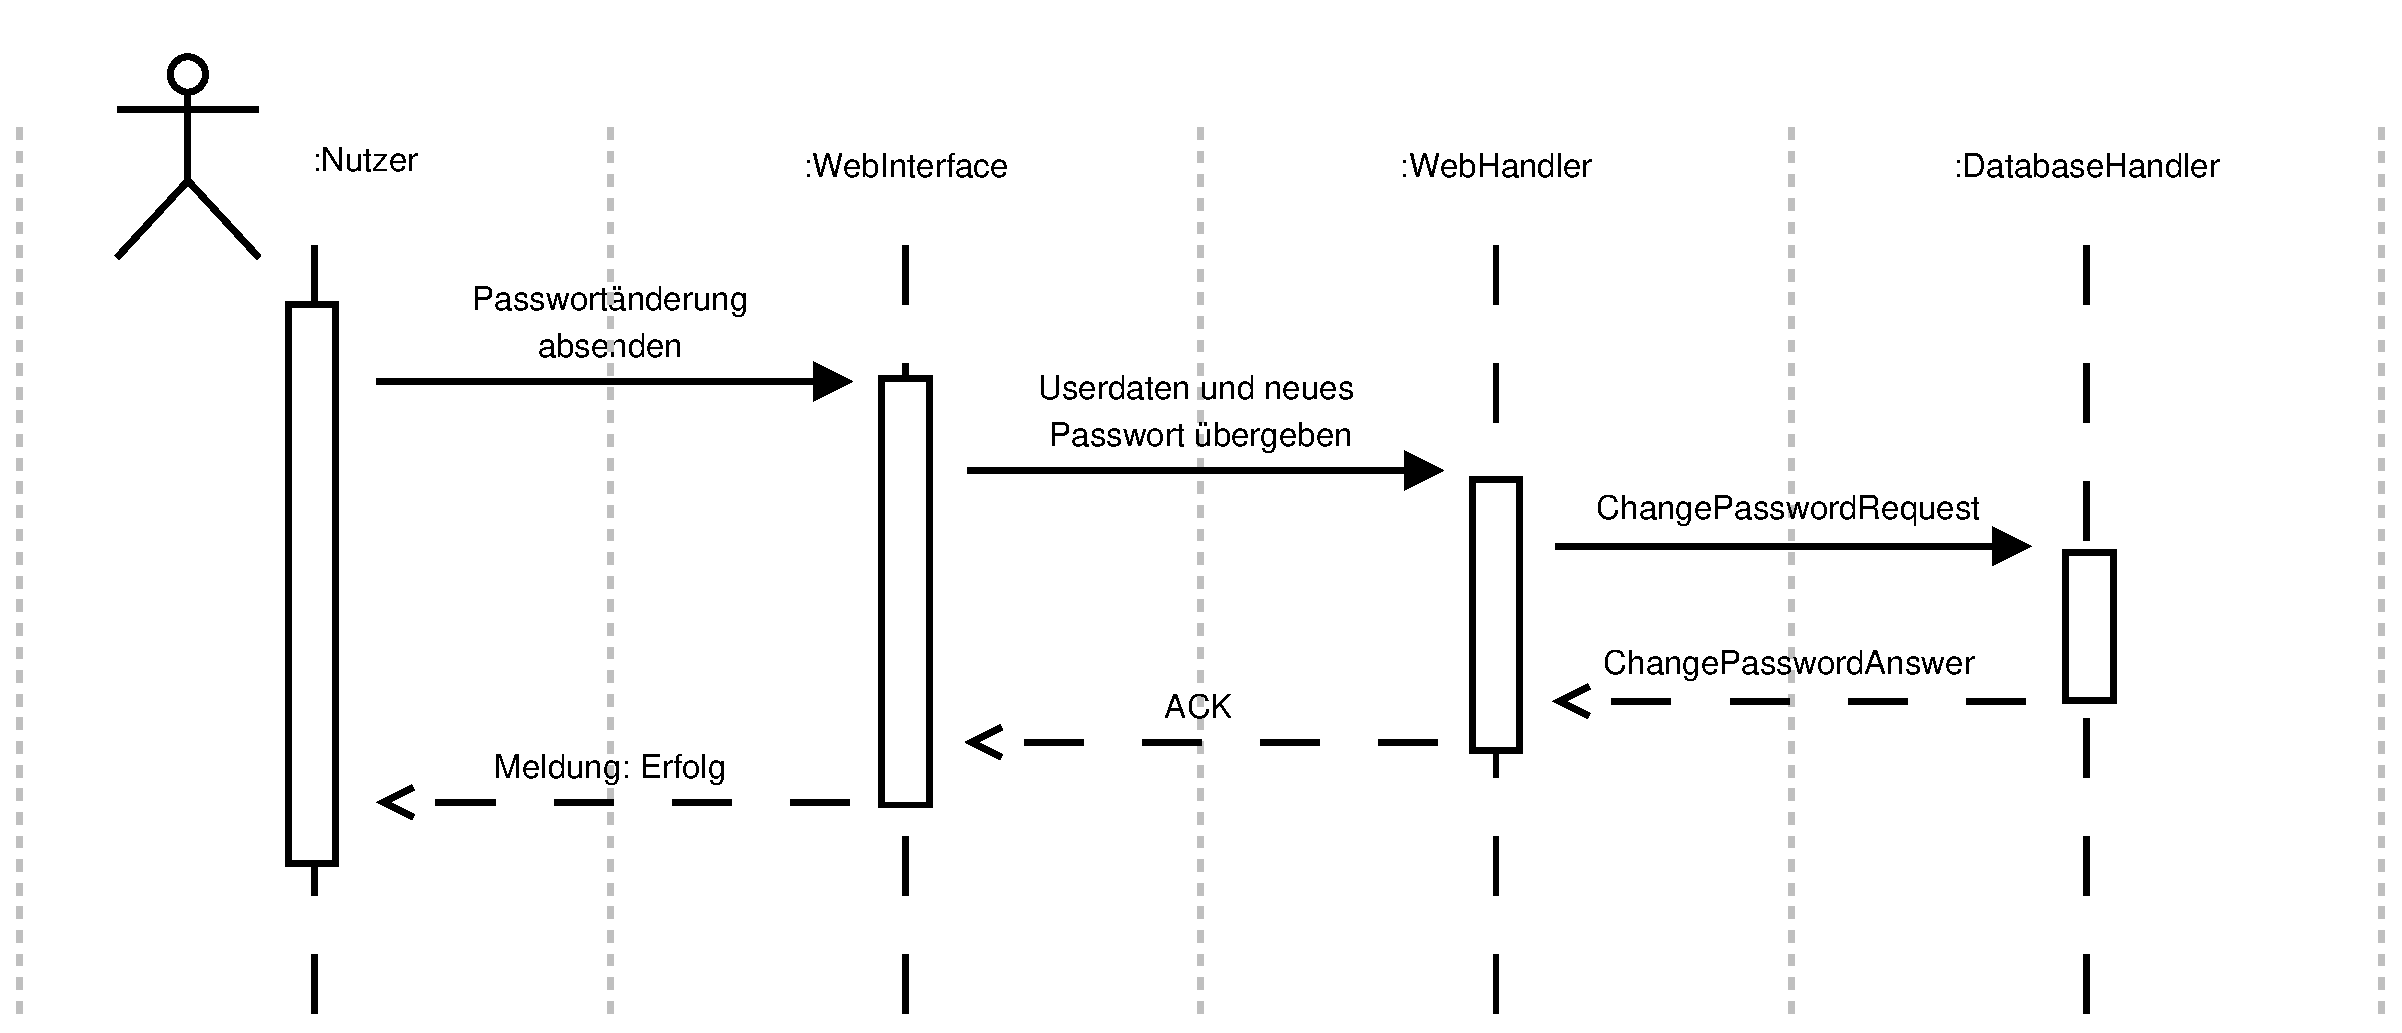
\includegraphics[width=1\textwidth]{Systementwurf/02_produktfunktionsanalyse/f800}
\caption{Sequenzdiagramm \textit{\ref{F80} Passwort ändern}
\label{sd80}}
\end{figure}


\section{Analyse von Funktionalität \ref{F81}: Passwort Wiederherstellung}

Das wiederherstellen eines Passworts ist dann nötig, wenn der Benutzer sein
Passwort vergessen hat. Er kann sich also nicht mehr im \textit{WebInterface}
einloggen. Deshalb wird auf der Login-Seite des \textit{WebInterface} ein Link
zu dieser Funktion eingebaut.

Sendet der Nutzer das Passwort-wiederherstellen-Formular im
\textit{WebInterface} unter Angabe seiner Emailadresse ab, wird diese an den
\textit{WebHandler} übertragen. Nun wird ein
\textit{RecoverPasswordRequest}-Objekt an den \textit{DatabaseHandler}
geschickt. Dieser prüft, ob ein Benutzer mit der eingegebenen Emailadresse
vorhanden ist. Ist dies der Fall, gibt er ein
\textit{RecoverPasswordAnswer}-Objekt mit einem Einmal-Link zu einem
Passwort-ändern-Formular zurück, welchen der \textit{WebHandler} per Email an
den Benutzer versendet.

Der Nutzer hat nun die Möglichkeit den in der Email erhaltenen Link aufzurufen
und wie in Abb.~\ref{sd81} gezeigt eine Passwort-ändern-Seite aufzurufen und
einmalig ohne eingeloggt zu sein die Funktion \ref{F80} zu nutzen.

\begin{figure}[h]
\centering
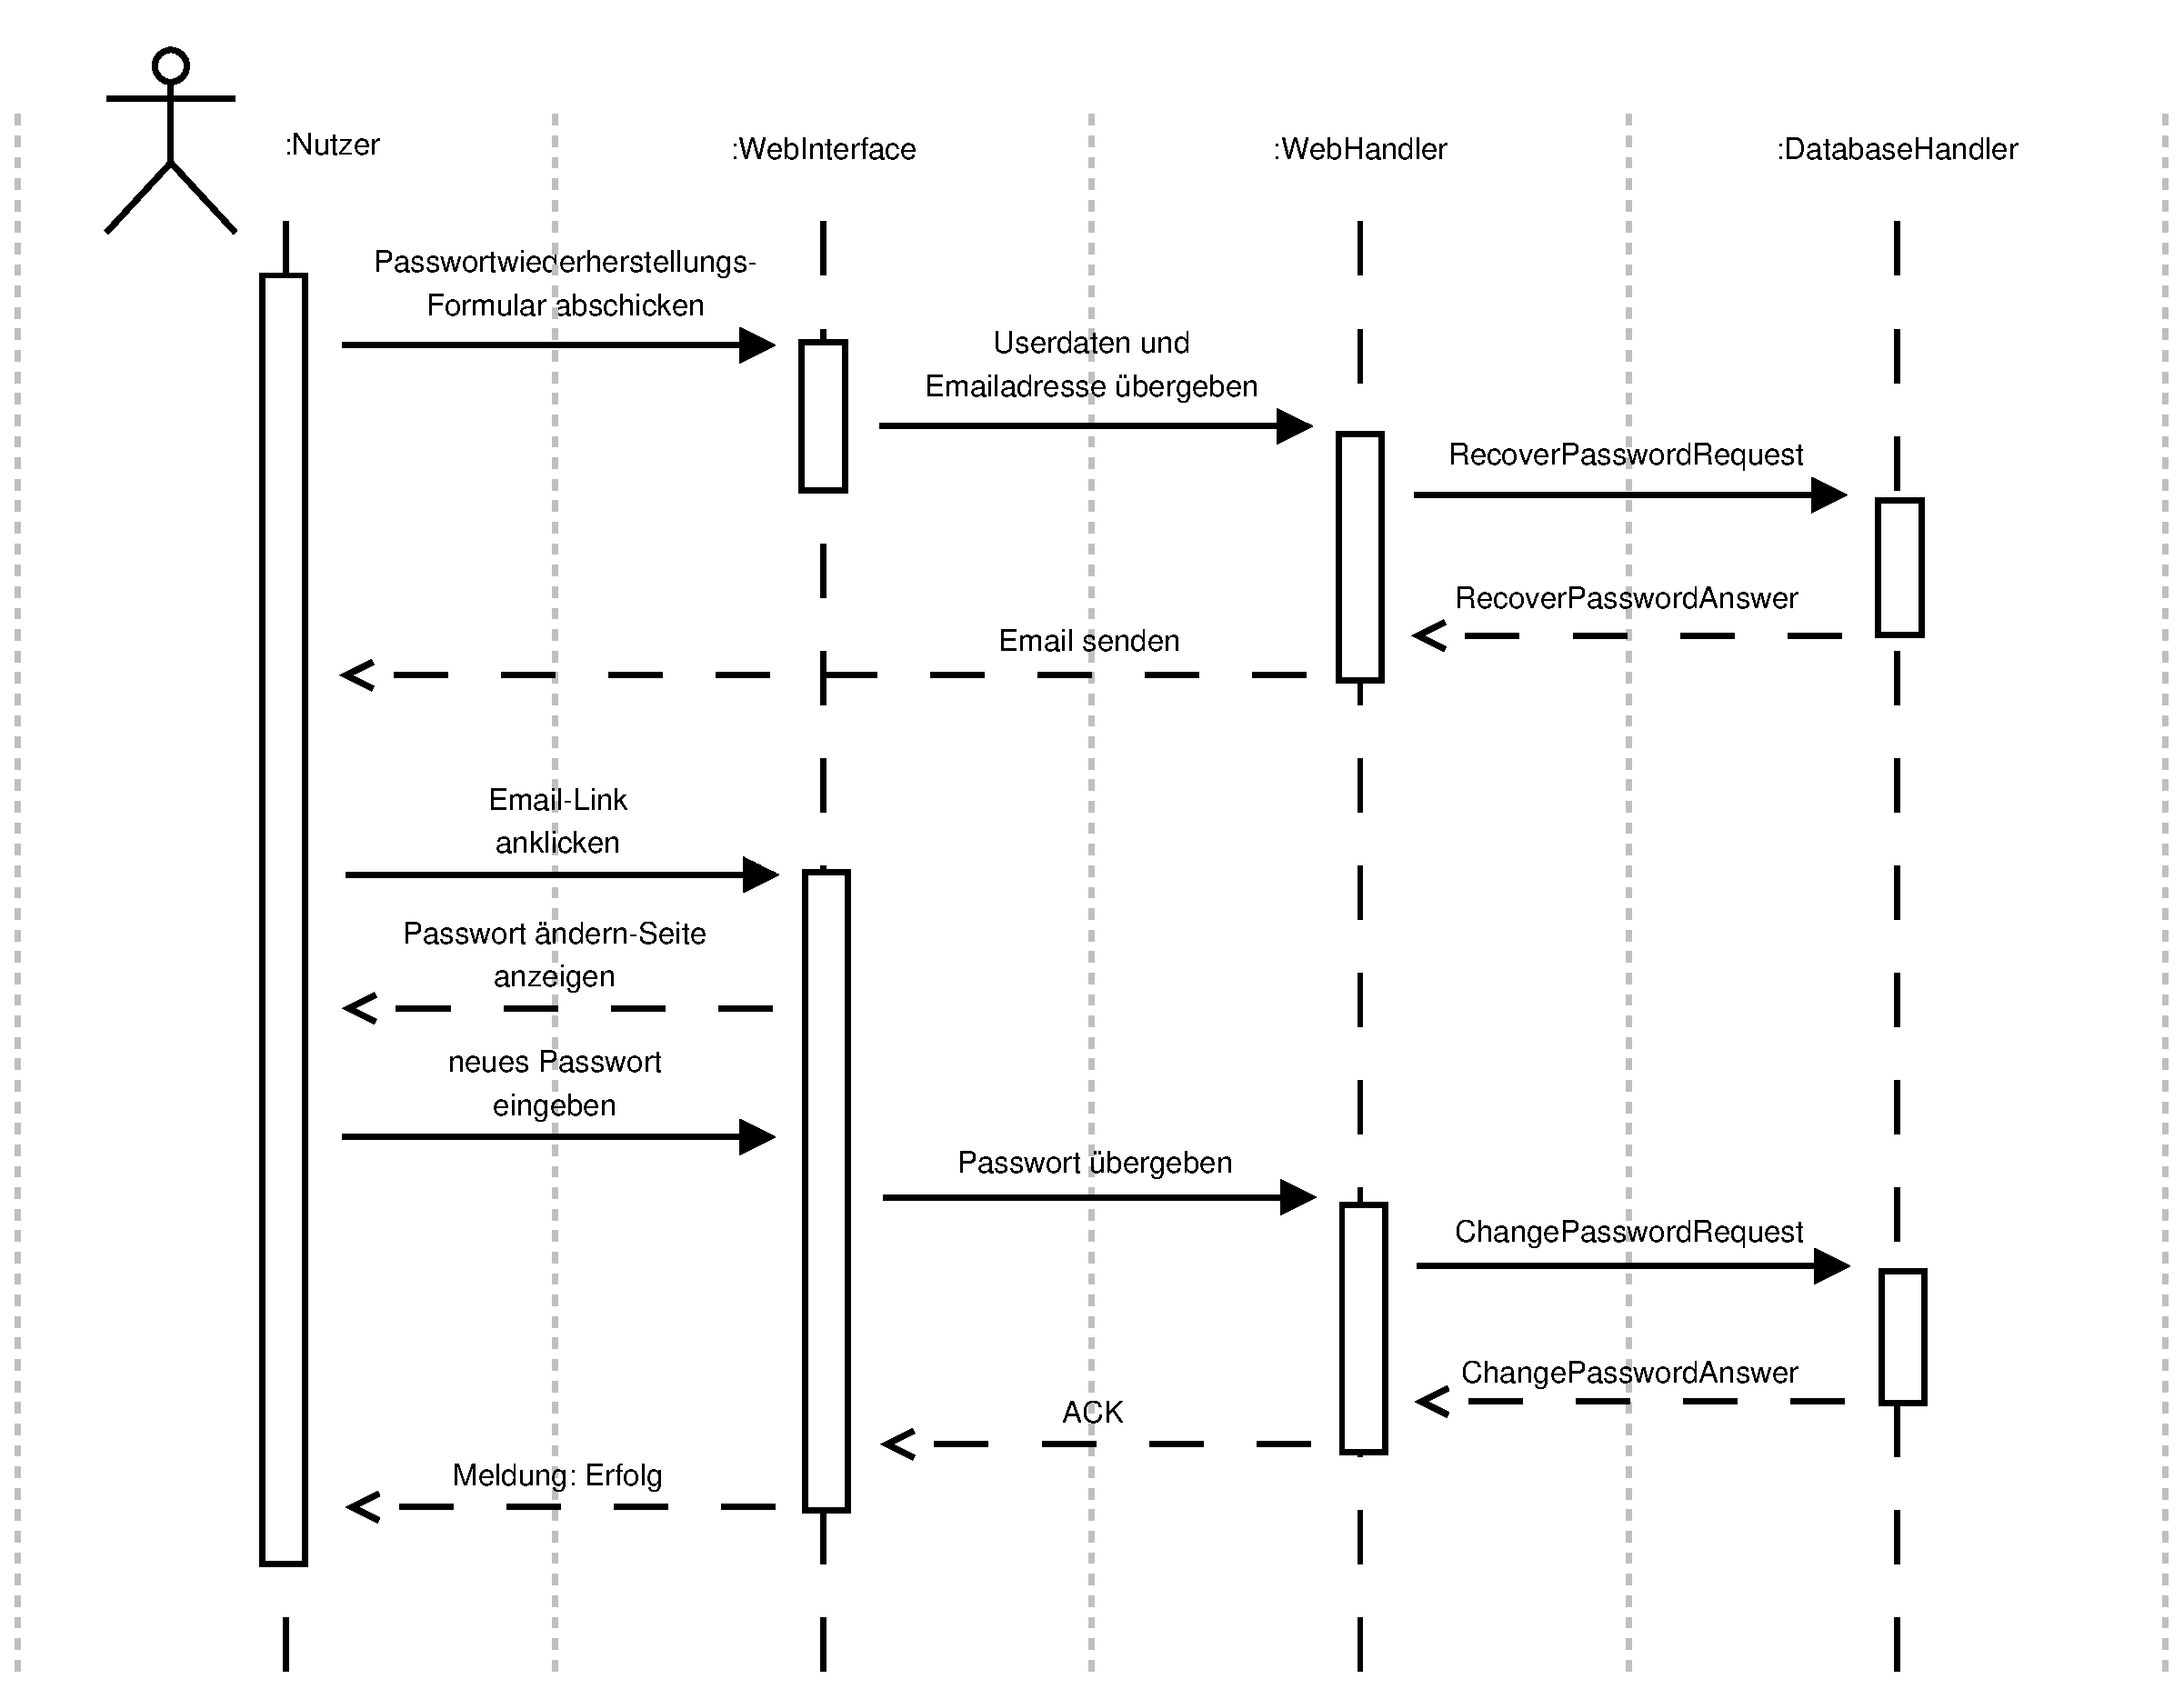
\includegraphics[width=1\textwidth]{Systementwurf/02_produktfunktionsanalyse/f810}
\caption{Sequenzdiagramm \textit{\ref{F81} Passwort Wiederherstellung}
\label{sd81}}
\end{figure}

\FloatBarrier

\section{Analyse von Funktionalität \ref{F90}: Rolle wechseln}

Hierbei handelt es sich um eine Funktion für Administratoren von \NewsGenie. Sie
erhalten so die Möglichkeit bei Problemen in die Rolle eines beliebigen
Benutzers zu wechseln und das \textit{WebInterface} so zu nutzen, als wären sie
als entsprechender Benutzer eingeloggt.

In Abb.~\ref{sd90} sieht man, dass dazu ein Link in der von \ref{F100}
angezeigten Liste neben dem jeweiligen Benutzer angeklickt werden kann, der den
\textit{WebHandler} anweist, das \textit{User}-Objekt des gewählten Benutzers
vom \textit{DatabaseHandler} abzurufen. Der \textit{WebHandler} ändert nun die
Session des Administrators so, dass er in die Rolle des Benutzers schlüpft. vom
\textit{WebHandler} wird anschließend eine Erfolgsmeldung über das
\textit{WebInterface} an den Benutzer gegeben.

\begin{figure}[h]
\centering
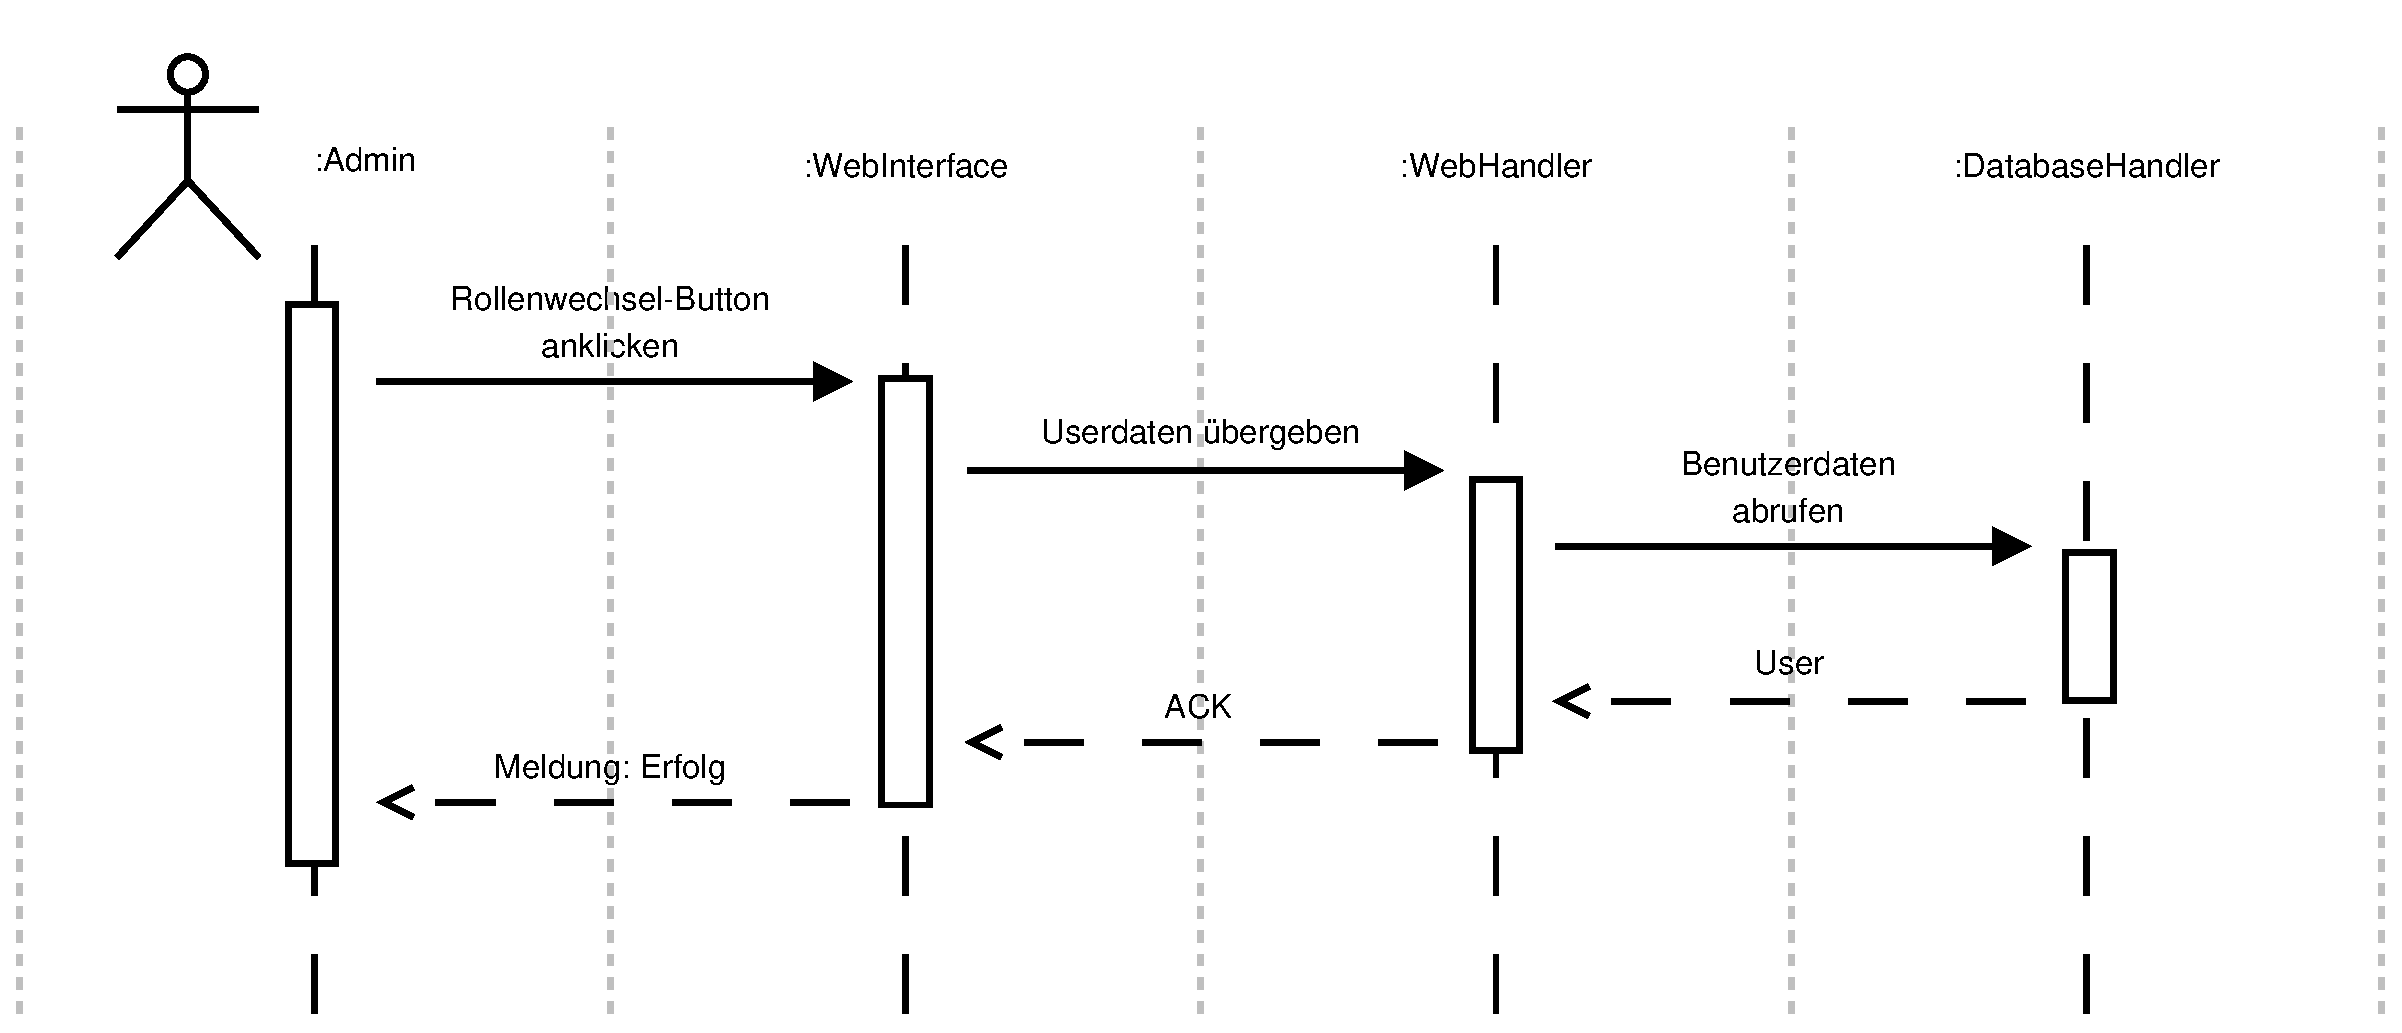
\includegraphics[width=1\textwidth]{Systementwurf/02_produktfunktionsanalyse/f900}
\caption{Sequenzdiagramm \textit{\ref{F90} Rolle wechseln}
\label{sd90}}
\end{figure}


\section{Analyse von Funktionalität \ref{F100}: Benutzerliste anzeigen}

Als Administrator hat man im \textit{WebInterface} die Möglichkeit eine Liste
aller Benutzer zu erhalten. In Abb.~\ref{sd100} ist zu sehen, dass Administrator
dazu im \textit{WebInterface} einen Button betätigt, woraufhin die Anforderung
der Benutzerliste an den \textit{WebHandler} übergeben wird. Dieser fordert
durch senden eines \textit{UserListRequest}-Objektes an den
\textit{DatabaseHandler} die Liste aus der Datenbank ab. Ein
\textit{UserListAnswer}-Objekt transportiert die Benutzerliste zurück an den
\textit{WebHandler}, welcher sie aufbereitet und an das \textit{WebInterface}
sendet, das sie dem Benutzer anzeigt.

\begin{figure}[h]
\centering
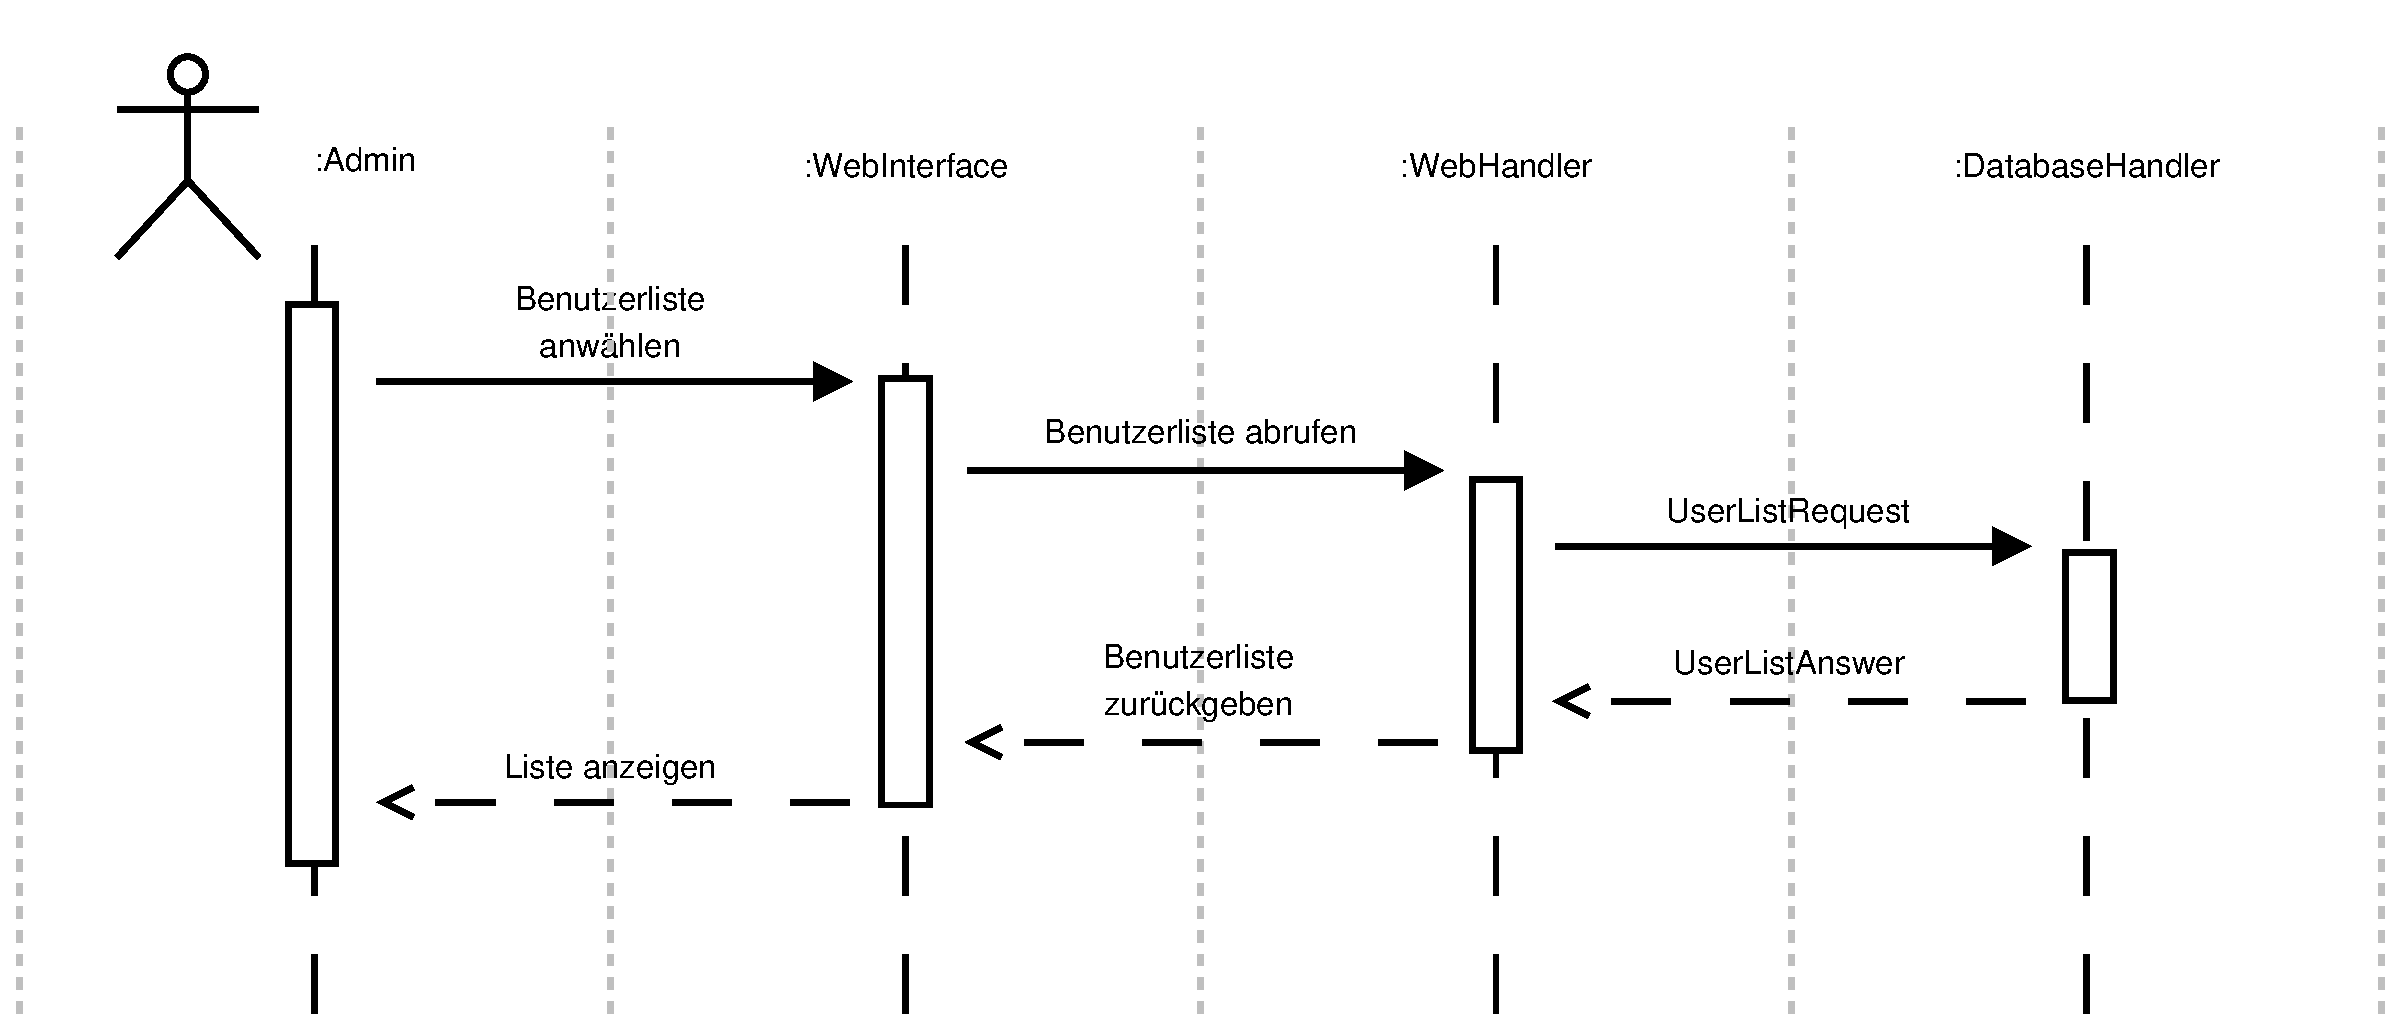
\includegraphics[width=1\textwidth]{Systementwurf/02_produktfunktionsanalyse/f1000}
\caption{Sequenzdiagramm \textit{\ref{F100} Benutzerliste anzeigen}
\label{sd100}}
\end{figure}

\FloatBarrier

\section{Analyse von Funktionalität \ref{F110}: Benutzer löschen}

Der Administrator hat weiterhin die Möglichkeit Benutzer von \NewsGenie
zu löschen. Dazu gibt es einen weiteren Button zu jedem Benutzer in der von
\ref{F100} ausgegebenen Benutzerliste.

Der Administrator betätigt den Löschen-Button des jeweiligen Benutzers wie in
Abb.~\ref{sd110} gezeigt und weißt damit das \textit{WebInterface} an, eine
Löschaufforderung an den \textit{WebHandler} zu senden. Dieser sendet ein
\textit{DeleteUserRequest}-Objekt an den \textit{DatabaseHandler}. Das Löschen
des Benutzers wird nun durch ein \textit{DeleteUserAnswer}-Objekt bestätigt und
vom \textit{WebHandler} eine Erfolgsmeldung über das \textit{WebInterface} an
den Benutzer gegeben.

\begin{figure}[h]
\centering
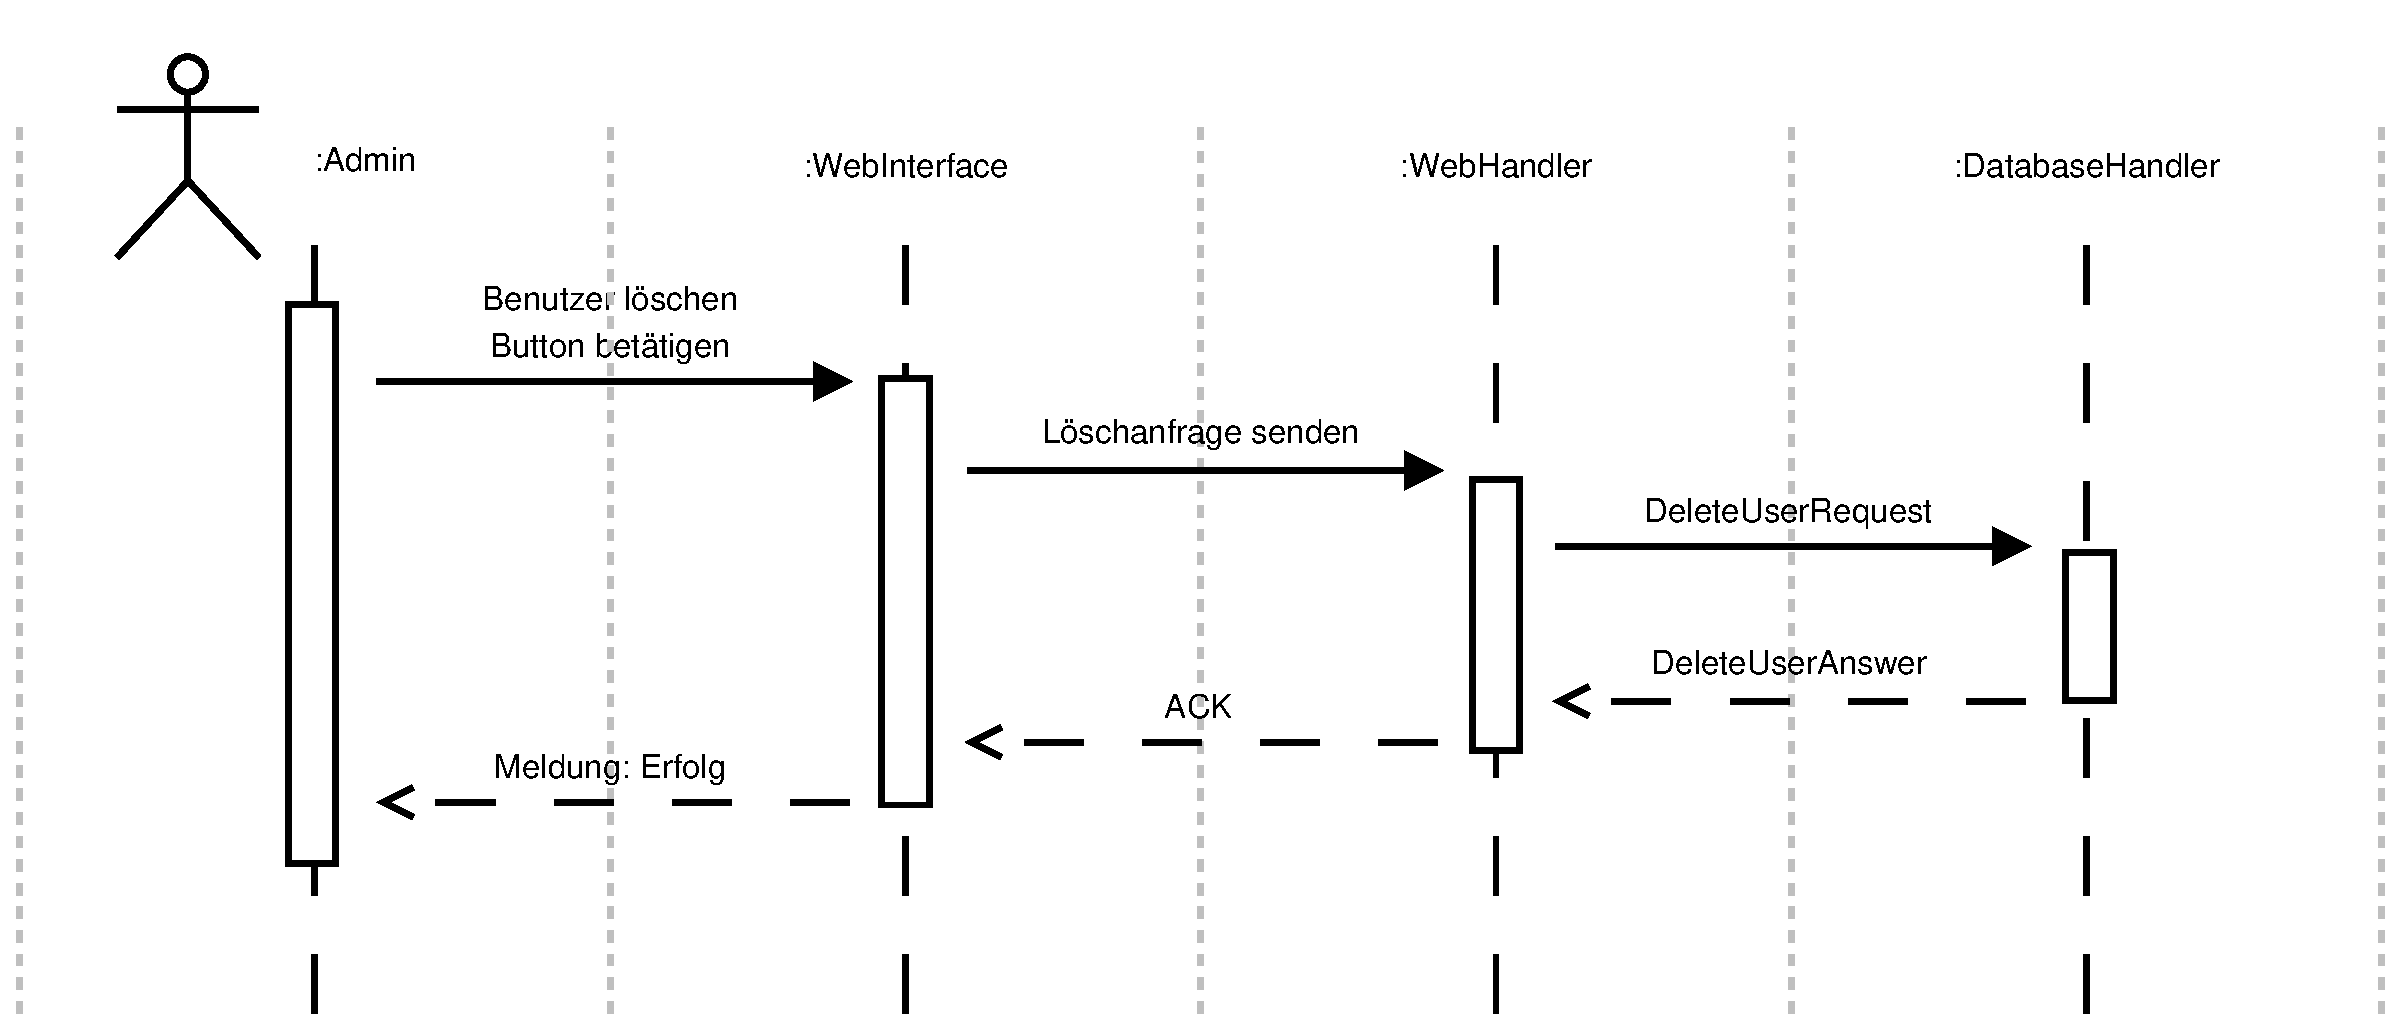
\includegraphics[width=1\textwidth]{Systementwurf/02_produktfunktionsanalyse/f1100}
\caption{Sequenzdiagramm \textit{\ref{F110} Benutzer löschen}
\label{sd110}}
\end{figure}


\section{Analyse von Funktionalität \ref{F120}: Text-Anfrage stellen}


Zu Analyse und Debug-Zwecken gibt es im \textit{WebInterface} außerdem die
Möglichkeit, als Nutzer direkt eine Anfrage an \NewsGenie einzugeben. So wird
die Spracherkennung und die Sprachausgabe des \textit{Client} aus der
Verarbeitung ausgeschlossen. Die Antwort wird wiederum im \textit{WebInterface}
zu lesen.

Abb.~\ref{sd120} zeigt, dass der Nutzer dazu im \textit{WebInterface} über ein
Formular eine Anfrage absenden kann, die vom \textit{WebHandler} an den
\textit{QueryProcessor} weitergereicht wird. Dieser analysiert die Anfrage und
ruft entsprechende Artikel durch senden eines \textit{SearchRequest}-Objektes an
den \textit{DatabaseHandler} ab. Als Antwort erhält er ein
\textit{SearchAnswer}-Objekt mit den entsprechenden Artikeln. Nun bereitet der
\textit{QueryProcessor} die Antwort in Satzform auf und sendet ein
\textit{ClientAnswer}-Objekt an den \textit{WebHandler} welcher die Antwort für
die Weitergabe an den Nutzer an das \textit{WebInterface} übergibt.

\begin{figure}[h]
\centering
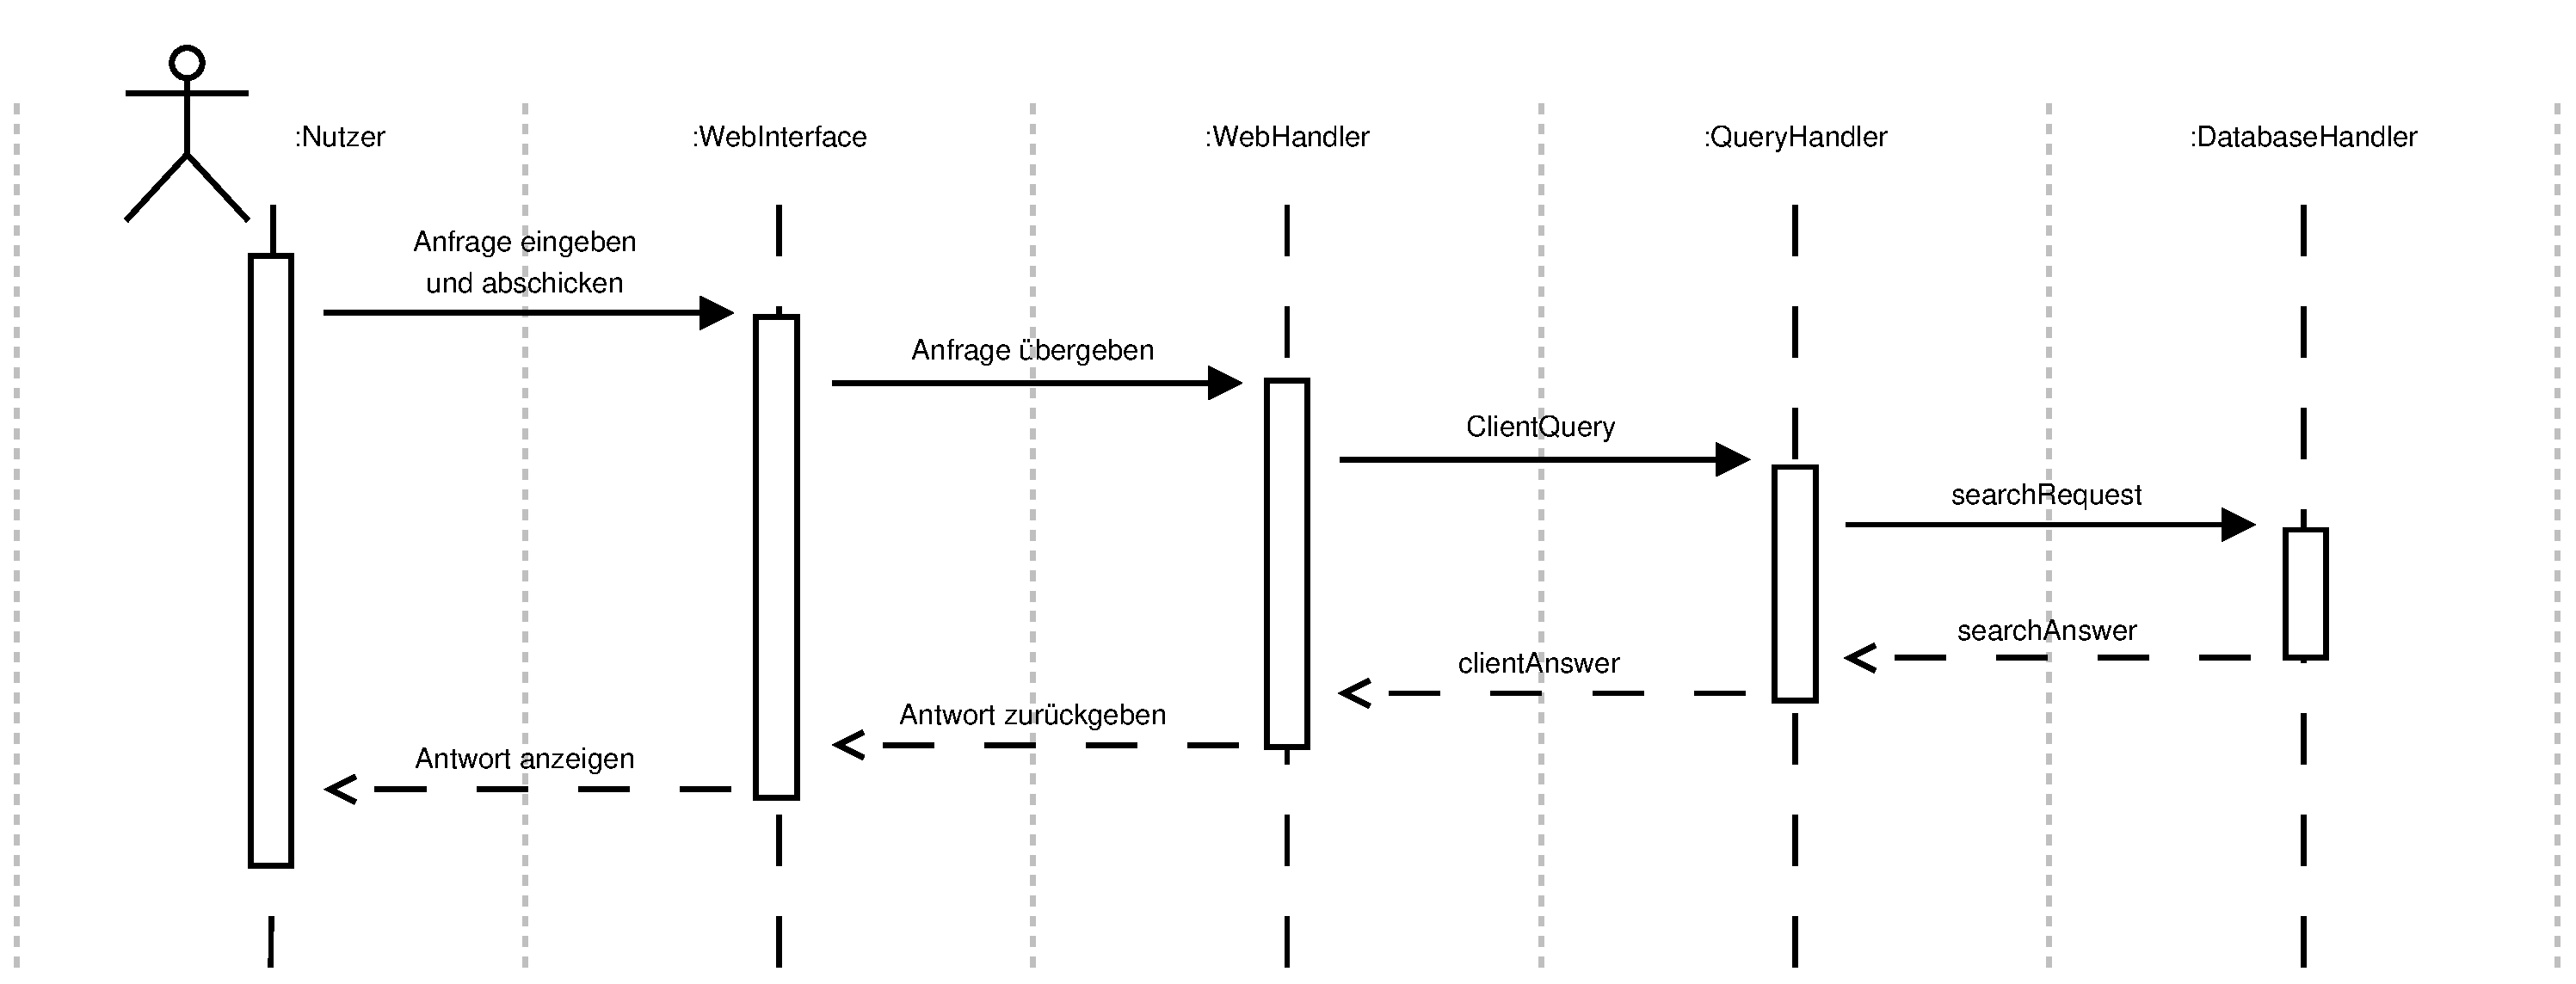
\includegraphics[width=1\textheight, angle=90]{Systementwurf/02_produktfunktionsanalyse/f1200}
\caption{Sequenzdiagramm \textit{\ref{F120} Text-Anfrage stellen}
\label{sd120}}
\end{figure}